% !TEX root = ../main.tex
\chapter{Thực nghiệm và Đánh giá}
\label{chap:experiment}

Chương này trình bày quá trình thực nghiệm nhằm kiểm chứng phương pháp đã đề xuất ở
Chương~\ref{chap:method}. Trước hết, chúng tôi mô tả môi trường, dữ liệu và cấu hình huấn
luyện (Mục~\ref{sec:exp-setup}--\ref{sec:exp-config}), cùng các độ đo được sử dụng
(Mục~\ref{sec:exp-metrics}). Phần kết quả được tổ chức theo hai câu hỏi nghiên cứu:
(1)~\textit{phương án khởi tạo nào là tốt nhất?} -- trả lời bằng thí nghiệm so sánh các
phương án khởi tạo trên cùng một lượng token huấn luyện (Mục~\ref{sec:exp-bakeoff}); và
(2)~\textit{mô hình cuối cùng đạt chất lượng ra sao so với các mô hình hiện có?} -- trả lời
bằng đường cong chất lượng theo ngân sách huấn luyện, bảng đánh giá đa tác vụ trên mười hai
tác vụ hiểu tiếng Việt, và kiểm chứng khả năng xử lý ngữ cảnh dài sau pha mở rộng lên 4.096 token
(Mục~\ref{sec:exp-mrc}). Cuối chương là phần thảo luận chung
(Mục~\ref{sec:exp-discussion}).

% ======================================================================
\section{Môi trường và dữ liệu thực nghiệm}
\label{sec:exp-setup}

Toàn bộ thực nghiệm được thực hiện trên GPU NVIDIA A100 (bộ nhớ 80GB, nền tảng Google
Colab), sử dụng PyTorch và hệ sinh thái Hugging Face (\texttt{transformers},
\texttt{datasets}, \texttt{safetensors}).

\subsection{Dữ liệu tiền huấn luyện}
\label{subsec:exp-cpt-data}

Giai đoạn căn chỉnh với phần thân đóng băng và tiếp tục tiền huấn luyện sử dụng phần tiếng Việt của
CulturaX~\cite{nguyen2023culturax} -- kho ngữ liệu web đa ngôn ngữ quy mô lớn đã được làm sạch
và khử trùng lặp. Tổng ngân sách xấp xỉ 5 tỷ token, tương đương khoảng 20GB văn bản.
Bảng~\ref{tab:data-stats} tóm tắt thống kê dữ liệu sử dụng trong đề tài.

\begin{table}[ht]
  \caption{Thống kê dữ liệu thực nghiệm.}
  \label{tab:data-stats}
  \centering
  \small
  \begin{tabular}{p{48mm}p{42mm}p{40mm}}
    \hline
    \textbf{Dữ liệu} & \textbf{Vai trò} & \textbf{Quy mô sử dụng} \\
    \hline
    CulturaX (tiếng Việt) & Căn chỉnh với phần thân đóng băng & $\sim$20 triệu token \\
    CulturaX (tiếng Việt) & Tiếp tục tiền huấn luyện & $\sim$5 tỷ token ($\sim$20GB văn bản) \\
    UIT-ViQuAD 2.0 (câu hỏi trả lời được) & Tinh chỉnh cho tác vụ ứng dụng & $\sim$18 nghìn câu hỏi huấn luyện \\
    Bộ đánh giá đa tác vụ (Mục~\ref{subsec:exp-eval-data}) & Tinh chỉnh cho tác vụ ứng dụng & 12 tác vụ: phân loại, suy luận, gán nhãn, tương đồng ngữ nghĩa, Retrieval, Reranking \\
    \hline
  \end{tabular}
\end{table}

\subsection{Dữ liệu đánh giá}
\label{subsec:exp-eval-data}

Mô hình được đánh giá trên một bộ tác vụ hiểu ngôn ngữ tiếng Việt đa dạng, bao quát các nhóm
năng lực khác nhau của một Encoder:

\begin{itemize}
  \item \textbf{Hỏi đáp đọc hiểu}: UIT-ViQuAD 2.0~\cite{nguyen2022vimrc} -- bộ dữ liệu hỏi
        đáp trích xuất xây dựng theo phương pháp luận của SQuAD; mô hình phải xác định đoạn văn bản trả lời
        trong ngữ cảnh cho trước. Chúng tôi chỉ dùng các câu hỏi \textit{trả lời được}
        (answerable); tập validation công khai được chia đôi ngẫu nhiên thành tập phát
        triển và tập kiểm tra.
  \item \textbf{Suy luận ngôn ngữ tự nhiên}: XNLI (phần tiếng Việt)~\cite{conneau2018xnli},
        ViANLI (bộ NLI đối kháng, khó hơn đáng kể)~\cite{huynh2024vianli} và QNLI bản tiếng
        Việt (suy luận câu hỏi--câu, phỏng theo GLUE~\cite{wang2018glue}).
  \item \textbf{Phân loại văn bản}: UIT-VSFC (phản hồi sinh viên)~\cite{nguyen2018vsfc},
        UIT-VSMEC (cảm xúc đa lớp)~\cite{ho2020vsmec}, UIT-ViCTSD (bình luận độc
        hại)~\cite{nguyen2021victsd}.
  \item \textbf{Tính chấp nhận được về ngữ pháp}: bộ dữ liệu kiểu CoLA~\cite{warstadt2019cola}
        cho tiếng Việt (ViCoLA-syn), trong đó câu sai ngữ pháp được sinh tự động từ câu đúng;
        mô hình phải phân biệt hai loại câu.
  \item \textbf{Gán nhãn chuỗi}: gán nhãn từ loại trên treebank Universal Dependencies
        Vietnamese-VTB~\cite{nguyen2009vtb}.
  \item \textbf{Tương đồng ngữ nghĩa}: bộ STS bản tiếng Việt~\cite{cer2017sts}, đo tương
        quan giữa điểm dự đoán và điểm do con người gán; và tác vụ phát hiện diễn đạt lại (paraphrase) --
        phân loại nhị phân cặp câu tương đương ngữ nghĩa xây dựng từ dữ liệu STS.
  \item \textbf{Biểu diễn câu (Retrieval và Reranking)}: Retrieval và Reranking xây dựng
        từ các cặp (câu hỏi, đoạn văn) của UIT-ViQuAD. Hai tác vụ này được đánh giá theo
        giao thức biểu diễn câu của NeoBERT cho MTEB~\cite{lebreton2025neobert}: lấy biểu
        diễn câu bằng gộp trung bình (mean pooling), rồi tinh chỉnh nhẹ bằng học tương phản
        (contrastive learning); quy trình này được áp dụng \textit{như nhau} cho mọi mô hình so sánh.
\end{itemize}

Bảng~\ref{tab:eval-tasks} tổng hợp toàn bộ bộ đánh giá cùng nhóm năng lực và độ đo
tương ứng của từng tác vụ.

\begin{table}[ht]
  \caption{Các tác vụ đánh giá.}
  \label{tab:eval-tasks}
  \centering
  \small
  \begin{tabular}{lll}
    \hline
    \textbf{Tác vụ (bộ dữ liệu)} & \textbf{Nhóm năng lực} & \textbf{Độ đo} \\
    \hline
    UIT-ViQuAD 2.0     & Hỏi đáp đọc hiểu        & EM, F1 ($\uparrow$) \\
    XNLI (vi)          & Suy luận ngôn ngữ       & Accuracy ($\uparrow$) \\
    ViANLI             & Suy luận đối kháng      & F1-macro ($\uparrow$) \\
    QNLI (vi)          & Suy luận câu hỏi--câu   & Accuracy ($\uparrow$) \\
    UIT-VSFC           & Phân loại phản hồi      & F1-weighted ($\uparrow$) \\
    UIT-VSMEC          & Phân loại cảm xúc       & F1-macro ($\uparrow$) \\
    UIT-ViCTSD         & Phân loại độc hại       & F1-macro ($\uparrow$) \\
    ViCoLA-syn         & Chấp nhận ngữ pháp      & MCC ($\uparrow$) \\
    UD-VTB             & Gán nhãn từ loại        & F1-macro ($\uparrow$) \\
    STS (vi)           & Tương đồng ngữ nghĩa    & Spearman ($\uparrow$) \\
    Paraphrase (STS)   & Phát hiện diễn đạt lại  & F1-macro ($\uparrow$) \\
    Retrieval (ViQuAD) & Biểu diễn câu           & nDCG@10 ($\uparrow$) \\
    Reranking (ViQuAD) & Biểu diễn câu           & MRR ($\uparrow$) \\
    \hline
  \end{tabular}
\end{table}

Bảng~\ref{tab:model-comparison} so sánh ViNeoBERT với các mô hình khác về quy mô tham số, dữ liệu tiếng Việt và độ dài ngữ cảnh.

\begin{table}[ht]
  \caption{Các mô hình Encoder được đánh giá.}
  \label{tab:model-comparison}
  \centering
  \small
  \resizebox{\textwidth}{!}{%
  \begin{tabular}{lcccc}
    \hline
    \textbf{Mô hình} & \textbf{Tham số} & \textbf{Kiến trúc} & \textbf{Dữ liệu tiếng Việt} & \textbf{Ngữ cảnh} \\
    \hline
    PhoBERT-base    & 135M & RoBERTa     & 20GB $\times$ 40 epoch $\approx$140B token & 512 \\
    PhoBERT-base-v2 & 135M & RoBERTa     & +120GB OSCAR-2301                           & 512 \\
    PhoBERT-large   & 370M & RoBERTa     & Cùng base (20GB)                            & 512 \\
    XLM-R-base      & 278M & RoBERTa     & $\approx$137GB CC-100 vi ($\approx$25B token vi) & 512 \\
    XLM-R-large     & 560M & RoBERTa     & Cùng base                                   & 512 \\
    \hline
    ViNeoBERT       & $\approx$250M & NeoBERT & 20GB, 1 lượt ($\approx$5B token) & 4.096 \\
    \hline
  \end{tabular}%
  }
\end{table}

% ======================================================================
\section{Cấu hình huấn luyện}
\label{sec:exp-config}

Bảng~\ref{tab:hyperparams} liệt kê siêu tham số của từng giai đoạn trong quy trình. Các
giá trị được giữ cố định cho \textit{mọi} phương án khởi tạo trong thí nghiệm so sánh, bảo
đảm khác biệt duy nhất giữa các phương án là cách khởi tạo lớp véc-tơ đầu vào và lớp đầu ra.

\begin{table}[ht]
  \caption{Siêu tham số huấn luyện.}
  \label{tab:hyperparams}
  \centering
  \small
  \resizebox{\textwidth}{!}{%
  \begin{tabular}{llll}
    \hline
    \textbf{Siêu tham số} & \textbf{Căn chỉnh với phần thân đóng băng} & \textbf{CPT (WSD)} & \textbf{Mở rộng ngữ cảnh} \\
    \hline
    Tốc độ học đỉnh        & $10^{-4}$        & $10^{-4}$          & $10^{-5}$ \\
    Khởi động (warmup)     & 10\% số bước     & 2\% (chặn $[20, 500]$ bước) & 50 bước \\
    Độ dài chuỗi tối đa    & 1.024            & 1.024              & 4.096 \\
    Batch size hiệu dụng   & $32 \times 4 = 128$ & $32 \times 16 = 512$ & $4 \times 32 = 128$ \\
    Tỷ lệ che MLM          & 20\%             & 20\%               & 20\% \\
    Bộ tối ưu              & \multicolumn{3}{c}{AdamW, $\beta = (0{,}9;\, 0{,}95)$, weight decay $0{,}01$} \\
    Lịch điều chỉnh tốc độ học & tuyến tính  & WSD, làm nguội theo CT~\ref{eq:wsd} & hằng số sau khởi động \\
    Số epoch               & 1 lượt ($\sim$20M token) & 1 lượt ($\sim$5 tỷ token) & 1 lượt ($\sim$200M token) \\
    \hline
  \end{tabular}%
  }
\end{table}

Đối với bước khởi tạo SALT, các siêu tham số chính gồm: số điểm neo kích hoạt tối đa qua
sparsemax là 64, ngưỡng số điểm neo tối thiểu cho ánh xạ cục bộ $k_0 = 8$, hệ số tỉ lệ trọng số
đầu ra $\gamma = 0{,}1$, và hệ số điều chỉnh đầu ra được ước lượng từ một mẫu CulturaX
khoảng 20 triệu token (Mục~\ref{sec:salt-proj}). Ở bước tinh chỉnh cho tác vụ ứng dụng, tác vụ
chính (hỏi đáp đọc hiểu) dùng AdamW với tốc độ học $2\times10^{-5}$, chuỗi tối đa 384,
batch 8, tối đa 5 epoch (dừng sớm); các tác vụ còn lại trong bộ đánh giá đa tác vụ được
tinh chỉnh theo quy trình tương tự với siêu tham số phù hợp từng tác vụ, giữ đồng nhất
giữa các mô hình so sánh.

% ======================================================================
\section{Độ đo đánh giá}
\label{sec:exp-metrics}

Chúng tôi sử dụng các nhóm độ đo sau; trừ khi ghi chú khác, mọi kết quả tinh chỉnh được
tính trung bình trên 5 lần chạy với các seed ngẫu nhiên (random seed) khác nhau và báo cáo kèm độ lệch chuẩn:

\begin{itemize}
  \item \textbf{Mất mát MLM và perplexity (PPL)($\downarrow$)}: mất mát cross-entropy của
        tác vụ mô hình hóa ngôn ngữ có mặt nạ trên tập giữ lại (held-out) của CulturaX, và
        perplexity tương ứng $\mathrm{PPL} = \exp(\mathcal{L}_{\mathrm{MLM}})$ -- dùng để
        theo dõi quá trình huấn luyện.
  \item \textbf{Exact Match (EM)($\uparrow$) và F1($\uparrow$)} cho hỏi đáp đọc hiểu: EM
        là tỷ lệ câu trả lời trùng khớp hoàn toàn với đáp án chuẩn sau chuẩn hóa; F1 đo
        mức chồng lấp ở cấp token giữa câu trả lời dự đoán và đáp án chuẩn.
  \item \textbf{Accuracy, F1-macro, F1-weighted ($\uparrow$)} cho các tác vụ phân loại và
        suy luận: F1-macro lấy trung bình đều giữa các lớp (phù hợp dữ liệu lệch lớp),
        F1-weighted lấy trung bình theo tỷ trọng lớp.
  \item \textbf{Hệ số tương quan Matthews (MCC)($\uparrow$)} cho tác vụ chấp nhận được về
        ngữ pháp: độ đo cân bằng cho phân loại nhị phân lệch lớp, nhận giá trị trong
        $[-1;\,1]$ -- quy ước chuẩn của bộ CoLA gốc.
  \item \textbf{Hệ số tương quan Spearman ($\uparrow$)} cho tác vụ tương đồng ngữ nghĩa:
        đo tương quan hạng giữa điểm dự đoán và điểm con người gán.
  \item \textbf{nDCG@10 ($\uparrow$) và MRR ($\uparrow$)} cho Retrieval và Reranking:
        nDCG@10 đánh giá chất lượng 10 kết quả đầu, ưu tiên kết quả đúng nằm ở thứ hạng cao
        (trọng số giảm dần theo vị trí); MRR là trung bình của nghịch đảo thứ hạng kết quả đúng.
        Hai tác vụ này chỉ chạy một lần theo giao thức biểu diễn câu chung nên không kèm độ lệch chuẩn.
\end{itemize}

Định nghĩa hình thức (công thức tường minh) của F1 ở cấp token, MCC, nDCG@$k$ và MRR được
trình bày trong Phụ lục~\ref{app:metrics}.

% ======================================================================
\section{So sánh các phương án khởi tạo}
\label{sec:exp-bakeoff}

Mục này gồm ba thí nghiệm được sắp xếp theo trình tự của quá trình khởi tạo để lựa chọn
cấu hình phù hợp nhất cho ViNeoBERT. Trước hết, Mục~\ref{subsec:exp-salt-geometry} kiểm
tra liệu kỹ thuật SALT có thực sự đưa các véc-tơ tiếng Việt vào vùng không gian mà phần
thân NeoBERT đã quen xử lý hay không. Sau đó, Mục~\ref{subsec:exp-gamma} xác định hệ số
tỉ lệ $\gamma$ cho ma trận đầu ra nhằm tạo ra điểm xuất phát ổn định. Cuối cùng,
Mục~\ref{subsec:exp-init-strategy} so sánh trực tiếp năm chiến lược khởi tạo trong cùng
điều kiện huấn luyện để lựa chọn phương án cuối. Theo cách tổ chức này, mỗi thí nghiệm
giải quyết một sai lệch cụ thể, lần lượt là vị trí của véc-tơ trong không gian biểu diễn,
độ lớn của tín hiệu đầu ra và hiệu quả tổng thể của toàn bộ chiến lược khởi tạo.

\subsection{Kiểm chứng hình học của kỹ thuật SALT}
\label{subsec:exp-salt-geometry}

Thí nghiệm đầu tiên được xây dựng từ thực tế rằng NeoBERT~\cite{lebreton2025neobert} đã
trải qua tiền huấn luyện, do đó phần thân mô hình đã quen tiếp nhận các véc-tơ có vị trí
và độ lớn nằm trong một phân phối nhất định. Khi thay lớp từ vựng bằng các token tiếng
Việt, các véc-tơ mới có thể nằm lệch khỏi phân phối này và trở thành loại đầu vào mà
NeoBERT chưa quen xử lý. Vì vậy, bài toán đặt ra là xác định liệu SALT~\cite{lee2025salt}
có đưa các véc-tơ tiếng Việt về đúng vùng không gian của NeoBERT hay không. Đầu vào của
thí nghiệm gồm hai tập véc-tơ 768 chiều tại thời điểm chưa tiếp tục huấn luyện: tập véc-tơ
tiếng Việt lấy từ ViDeBERTa~\cite{lai2023videberta} và tập véc-tơ gốc của NeoBERT. Từ hai
tập đầu vào này, thí nghiệm tạo ra hình PCA hai chiều trước và sau SALT, đồng thời đo
khoảng cách giữa tâm của hai đám mây véc-tơ. Đầu ra này cho phép kiểm tra trực quan rằng
khoảng cách càng nhỏ và độ trải càng giống nhau thì lớp từ vựng tiếng Việt càng gần với
phân phối mà phần thân NeoBERT đã quen xử lý.

\begin{figure}[ht]
  \centering
  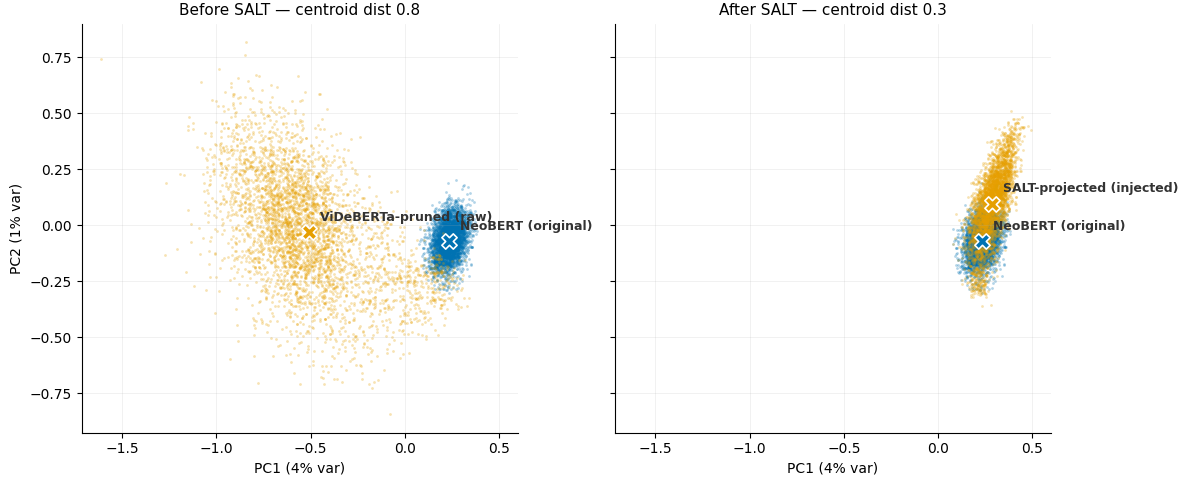
\includegraphics[width=\textwidth]{images/beforeandaftersalt.png}
  \caption{Lớp véc-tơ tiếng Việt trước và sau khi áp dụng SALT.}
  \label{fig:salt-before-after}
\end{figure}

Trong Hình~\ref{fig:salt-before-after}, mỗi điểm biểu diễn véc-tơ của một token, trong đó
màu vàng tương ứng với các token tiếng Việt, màu xanh tương ứng với các token của NeoBERT
và dấu $\times$ biểu diễn tâm của từng đám mây. Do mỗi véc-tơ có 768 chiều nên không thể
quan sát trực tiếp; PCA được sử dụng để chiếu chúng xuống hai chiều PC1 và PC2, lần lượt
giữ khoảng 4\% và 1\% mức biến thiên. Tỉ lệ này nhỏ là bình thường trong không gian nhiều
chiều, còn yếu tố quan trọng là cả hai tập véc-tơ được biểu diễn trên cùng một hệ trục,
nhờ đó vị trí tương đối của chúng có thể được so sánh trực tiếp. Các token điểm neo và
token đặc biệt không được hiển thị trong hình vì chúng được sao chép trực tiếp từ NeoBERT;
nếu giữ lại, những điểm vốn đã trùng nhau này sẽ tạo ra vùng chồng lấp giả và làm mức độ
khớp giữa hai tập véc-tơ có vẻ tốt hơn thực tế.

Trước khi áp dụng SALT, thể hiện ở biểu đồ bên trái của
Hình~\ref{fig:salt-before-after}, đám mây màu vàng nằm lệch và trải rộng hơn rõ rệt so với
đám mây màu xanh, với khoảng cách giữa hai tâm là 0,8. Kết quả này cho thấy lớp từ vựng
tiếng Việt đang tạo ra một phân phối đầu vào khác với phân phối mà NeoBERT đã tiếp xúc
trong tiền huấn luyện, không chỉ về vị trí mà còn về độ lớn. Nếu các véc-tơ này được đưa
trực tiếp vào mô hình, sai lệch ban đầu có thể tiếp tục bị khuếch đại qua 28 lớp
Pre-RMSNorm (Mục~\ref{subsec:rmsnorm}).

Sau khi áp dụng SALT, thể hiện ở biểu đồ bên phải của
Hình~\ref{fig:salt-before-after}, đám mây màu vàng chồng lấp nhiều hơn với đám mây màu
xanh, khoảng cách giữa hai tâm giảm từ 0,8 xuống 0,3 và độ trải của chúng cũng trở nên
tương đồng hơn. Có thể hiểu rằng SALT đã điều chỉnh hướng của véc-tơ tiếng Việt để đưa
chúng về vùng mà phần thân NeoBERT quen xử lý, trong khi bước hiệu chỉnh độ lớn
(Mục~\ref{subsec:norm-calib}) đưa độ lớn của chúng về mức phù hợp. Một phần đuôi màu vàng
vẫn còn lệch nhẹ, chủ yếu gồm các token hiếm, và tiếp tục được điều chỉnh trong pha căn
chỉnh với phần thân đóng băng (Mục~\ref{sec:freeze}).

Như vậy, Hình~\ref{fig:salt-before-after} xác nhận SALT đã thực hiện đúng vai trò hình học
của phương pháp: đưa lớp véc-tơ tiếng Việt từ một phân phối lệch về gần vùng không gian
của NeoBERT. Khoảng cách tâm giảm từ 0,8 xuống 0,3 và độ trải trở nên tương đồng hơn; kết
quả này cũng phù hợp với mất mát MLM ngay sau SALT là 7,21, thấp hơn đáng kể so với mức
khởi tạo ngẫu nhiên trên 10.

\subsection{Lựa chọn hệ số tỉ lệ trọng số đầu ra}
\label{subsec:exp-gamma}

Kết quả ở Mục~\ref{subsec:exp-salt-geometry} cho thấy SALT đã đưa các véc-tơ tiếng Việt
về gần không gian mà phần thân NeoBERT quen xử lý. Tuy nhiên, đối với ma trận đầu ra,
việc nằm đúng hướng ngữ nghĩa chưa bảo đảm rằng điểm dự đoán ban đầu có độ lớn phù hợp;
vì vậy, thí nghiệm thứ hai lựa chọn hệ số $\gamma$ để điều chỉnh ảnh hưởng của ma trận
này sau SALT. Theo Công thức~\eqref{eq:dec-scale},
$y = \gamma W_{\mathrm{dec}}h + b_{\mathrm{dec}}$, trong đó $h$ là biểu diễn ngữ cảnh,
$y$ là véc-tơ điểm số trước hàm softmax, $W_{\mathrm{dec}}h$ là phần điểm số theo ngữ
cảnh do ma trận SALT tạo ra, còn $b_{\mathrm{dec}}$ chứa log-tần suất token tiếng Việt.
Do $W_{\mathrm{dec}}$ mới được khởi tạo và chưa được căn chỉnh với phần thân NeoBERT
trên dữ liệu tiếng Việt, biên độ của $W_{\mathrm{dec}}h$ có thể quá lớn và lấn át tác
dụng của $b_{\mathrm{dec}}$ ở những bước đầu. Do đó, $\gamma$ cần đủ nhỏ để
$b_{\mathrm{dec}}$ phát huy tác dụng nhưng vẫn khác 0 để giữ lại hướng ngữ nghĩa do SALT
chuyển giao. Thí nghiệm giữ nguyên toàn bộ cấu hình, chỉ thay đổi
$\gamma \in \{0{,}1;\,0{,}5;\,1{,}0\}$, rồi so sánh đường mất mát MLM theo số bước huấn
luyện trong Hình~\ref{fig:gamma-loss}.

\begin{figure}[ht]
  \centering
  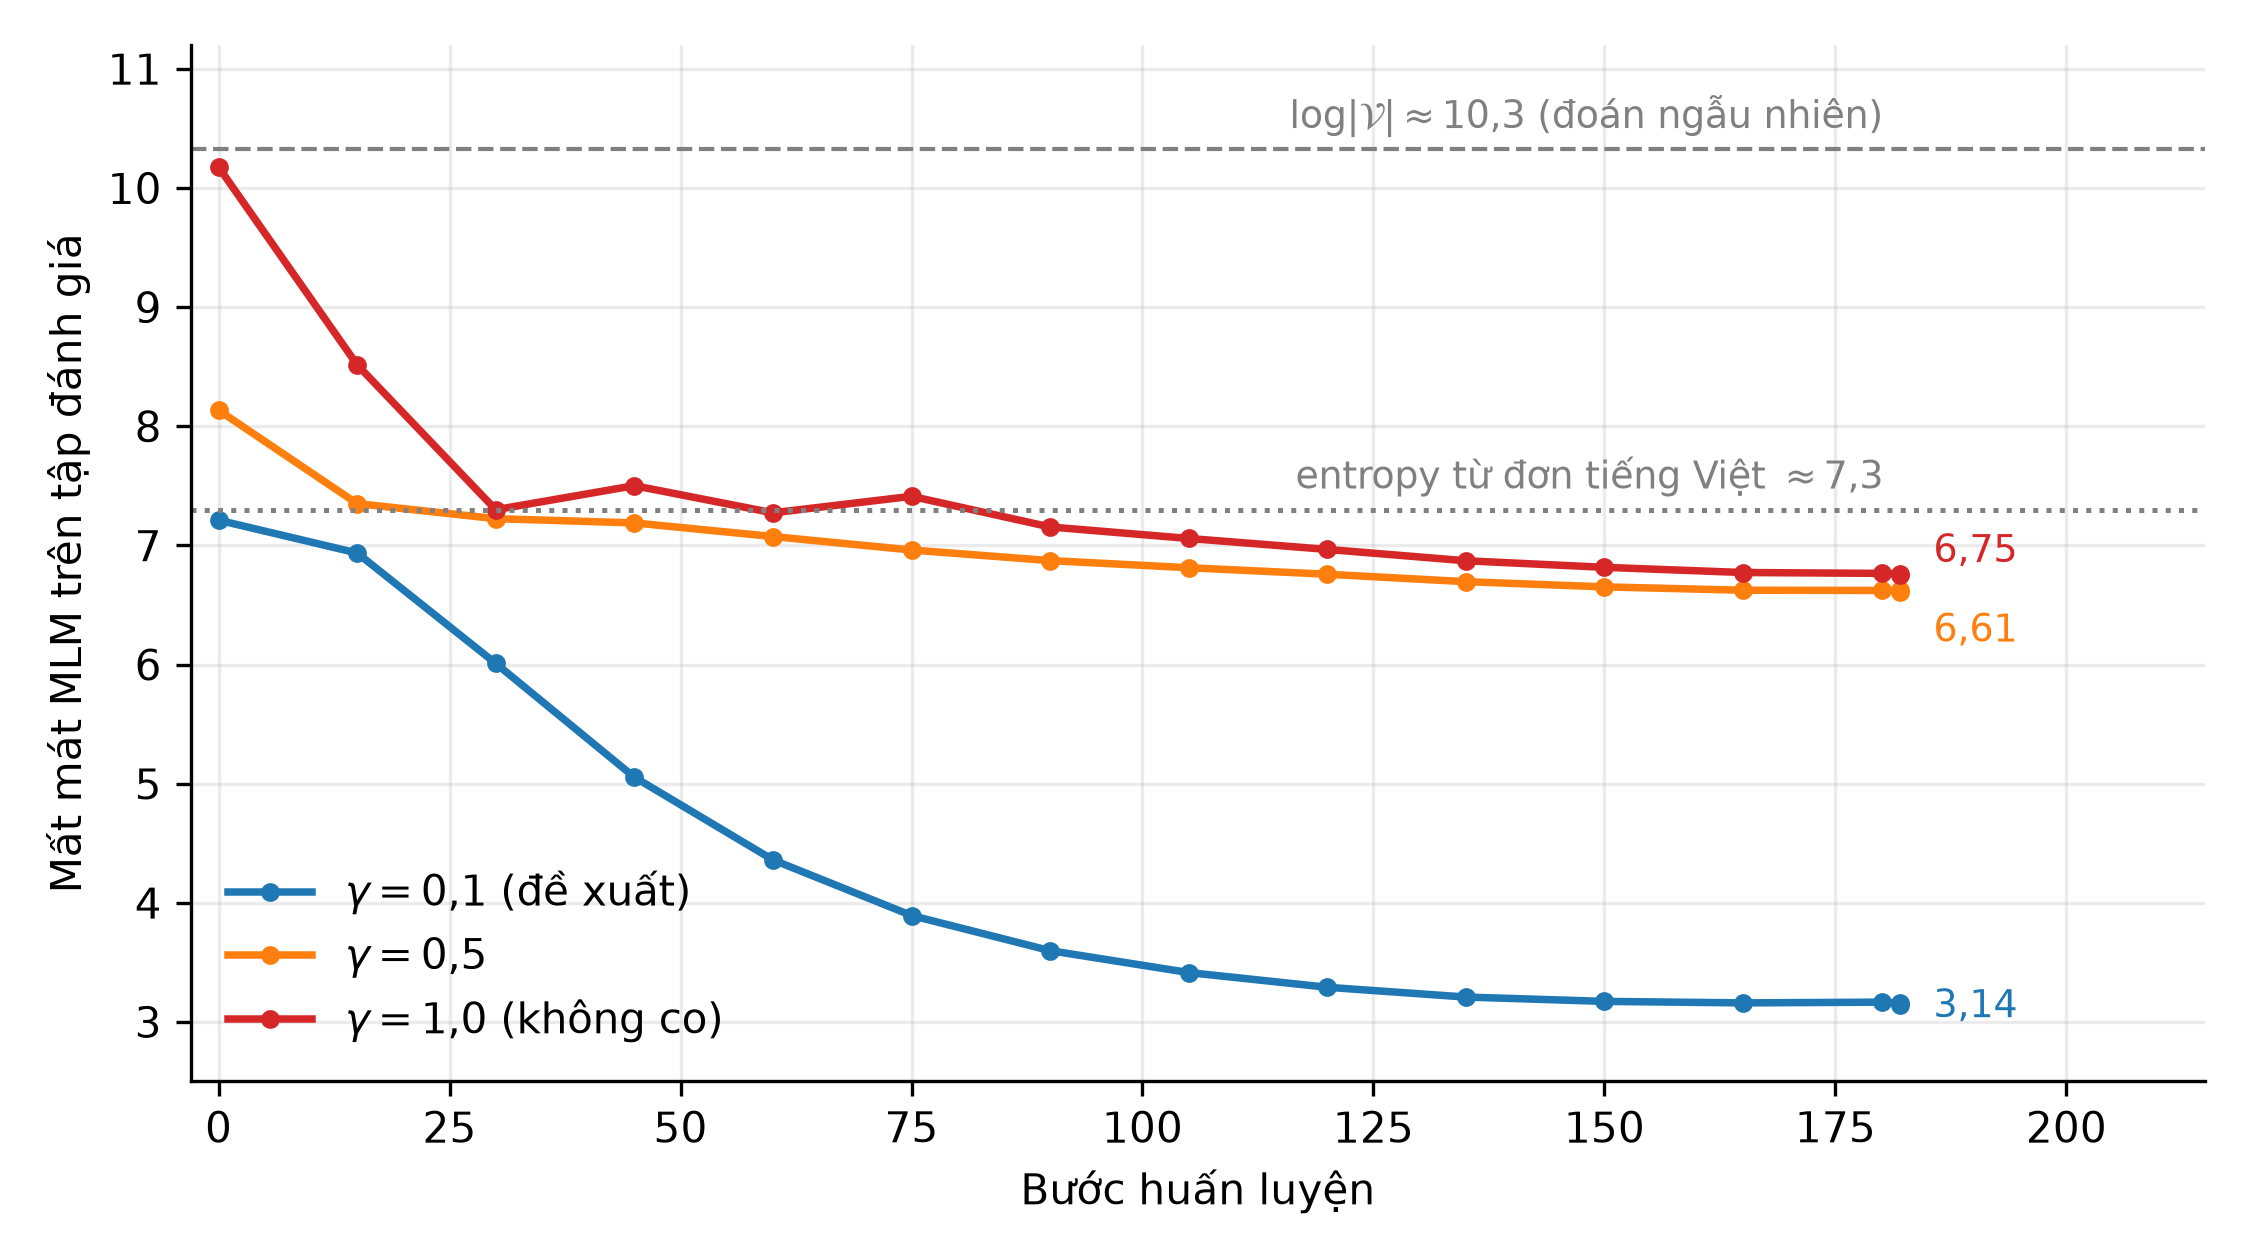
\includegraphics[width=0.92\textwidth]{images/gamma_scale_loss.png}
  \caption{Mất mát MLM theo hệ số tỉ lệ $\gamma$.}
  \label{fig:gamma-loss}
\end{figure}

Hình~\ref{fig:gamma-loss} sử dụng trục ngang để biểu diễn số bước huấn luyện và trục dọc
để biểu diễn mất mát MLM trên tập đánh giá, do đó đường cong càng thấp thì kết quả càng
tốt. Đường xanh tương ứng với $\gamma = 0{,}1$, đường cam tương ứng với
$\gamma = 0{,}5$ và đường đỏ tương ứng với $\gamma = 1{,}0$. Đường tham chiếu ở khoảng
7,3 là entropy unigram tiếng Việt, tức mức mất mát kỳ vọng khi dự đoán ban đầu chủ yếu
dựa trên $b_{\mathrm{dec}}$ và tần suất xuất hiện của token; đường tham chiếu ở khoảng
10,3 là mức dự đoán ngẫu nhiên $\log|\mathcal{V}_t|$. Hai mốc này cho biết thành phần
nào trong Công thức~\eqref{eq:dec-scale} đang chi phối dự đoán ở thời điểm khởi tạo.

Với $\gamma = 1{,}0$, $W_{\mathrm{dec}}h$ được giữ nguyên biên độ nên các điểm số theo
ngữ cảnh chưa được căn chỉnh lấn át $b_{\mathrm{dec}}$; mô hình khởi đầu ở mức mất mát
10,18, gần dự đoán ngẫu nhiên 10,3, chuẩn gradient ban đầu lên tới 68,4 và mất mát sau
đó chỉ dừng quanh 6,75. Khi $\gamma$ giảm xuống 0,5, ảnh hưởng của
$W_{\mathrm{dec}}h$ đã nhỏ hơn nhưng vẫn đủ lớn để che lấp đáng kể tín hiệu tần suất;
mức mất mát khởi đầu còn 8,13, chuẩn gradient là 15,8 và đường cong vẫn sớm mắc quanh
6,61. Ngược lại, với $\gamma = 0{,}1$, thành phần $\gamma W_{\mathrm{dec}}h$ được thu
nhỏ đủ để $b_{\mathrm{dec}}$ chi phối dự đoán ban đầu, vì vậy mất mát khởi đầu là 7,21,
gần entropy unigram tiếng Việt, và chuẩn gradient chỉ còn 2,1. Do $\gamma$ vẫn khác 0,
hướng ngữ nghĩa của $W_{\mathrm{dec}}$ không bị loại bỏ; từ điểm xuất phát ổn định này,
mô hình tiếp tục học thông tin ngữ cảnh và giảm mất mát xuống 3,14.

Kết quả cho thấy vai trò của $\gamma$ không phải là loại bỏ ảnh hưởng của SALT mà là cân
bằng hai thành phần trong Công thức~\eqref{eq:dec-scale}. Giá trị $\gamma = 0{,}1$ làm
giảm biên độ của phần điểm số ngữ cảnh chưa ổn định, nhờ đó $b_{\mathrm{dec}}$ đã chứa
log-tần suất tiếng Việt có thể phát huy tác dụng tối đa ở những bước đầu; đồng thời, phép
nhân với một số khác 0 vẫn bảo toàn hướng ngữ nghĩa mà SALT đã tạo ra. Vì đáp ứng được
cả hai yêu cầu này và cho đường hội tụ tốt nhất, $\gamma = 0{,}1$ được lựa chọn cho toàn
bộ các thí nghiệm tiếp theo.

\subsection{Lựa chọn chiến lược khởi tạo ma trận từ vựng}
\label{subsec:exp-init-strategy}

Sau khi xác nhận SALT có thể đưa véc-tơ về đúng vùng và $\gamma = 0{,}1$ tạo ra điểm
xuất phát ổn định, thí nghiệm cuối cùng kiểm tra liệu hướng ngữ nghĩa được SALT chuyển
giao có thực sự tốt hơn các cách khởi tạo ngẫu nhiên, việc dùng chung trọng số có phù hợp
hay không và pha căn chỉnh với phần thân đóng băng có mang lại lợi ích bổ sung hay không.
Để trả lời các câu hỏi này, năm chiến lược khởi tạo được xây dựng với mức độ tận dụng
thông tin từ mô hình nguồn tăng dần như sau.

\begin{itemize}
  \item \textbf{Ngẫu nhiên ngây thơ (Naive random)}: cả ma trận véc-tơ đầu vào và ma trận
        đầu ra đều được khởi tạo lại theo phân phối $\mathcal{N}(0;\,0{,}02)$, còn hệ số
        điều chỉnh theo tần suất được đặt bằng 0. Phương án này không sử dụng bất kỳ thông
        tin nào từ không gian véc-tơ nguồn và đóng vai trò là mốc sàn.
  \item \textbf{Ngẫu nhiên khớp mô-men (Norm-matched random)}: mỗi hàng từ vựng mới vẫn
        có hướng ngẫu nhiên nhưng được co giãn về đúng độ lớn trung bình của lớp véc-tơ
        NeoBERT; ma trận đầu ra được suy ra từ lớp véc-tơ đầu vào qua cùng ánh xạ tuyến
        tính toàn cục và sử dụng cùng hệ số điều chỉnh theo tần suất như SALT. Phương án
        này khớp SALT ở các thành phần phụ trợ nhưng không mang hướng ngữ nghĩa từ mô hình
        nguồn.
  \item \textbf{Dùng chung trọng số (Weight tying)}: ma trận đầu ra được sao chép trực
        tiếp từ ma trận véc-tơ đầu vào tại thời điểm khởi tạo. Đây là cách làm thường gặp
        ở các kiến trúc buộc hai lớp dùng chung trọng số, nhưng NeoBERT gốc không sử dụng
        cơ chế này.
  \item \textbf{SALT cho hai ma trận (nhãn ``SALT (both)'')}: kỹ thuật SALT được áp dụng
        riêng theo từng token cho cả ma trận véc-tơ đầu vào và ma trận đầu ra, đồng thời
        sử dụng $\gamma = 0{,}1$ (Mục~\ref{subsec:both-matrices}). Hai ma trận vì vậy
        cùng kế thừa cấu trúc ngữ nghĩa nhưng vẫn được phép đảm nhiệm hai vai trò hình học
        khác nhau.
  \item \textbf{SALT kết hợp căn chỉnh phần thân đóng băng (nhãn ``SALT + freeze'')}:
        giữ nguyên cách khởi tạo của SALT (both), sau đó bổ sung pha huấn luyện khoảng
        20 triệu token chỉ cập nhật hai ma trận từ vựng trong khi toàn bộ phần thân
        NeoBERT được đóng băng trước khi tiếp tục tiền huấn luyện
        (Mục~\ref{sec:freeze}).
\end{itemize}

Cả năm chiến lược trên được tiếp tục tiền huấn luyện trong cùng cấu hình tới mốc khoảng
100 triệu token. Đầu ra của thí nghiệm được báo cáo theo hai tiêu chí song song trong
Hình~\ref{fig:init-strategy}: mất mát MLM/PPL trên tập đánh giá và điểm F1 trên
UIT-ViQuAD. Mất mát và PPL càng thấp thì khả năng dự đoán token càng tốt, trong khi F1
càng cao thì biểu diễn càng hữu ích cho bài toán đọc hiểu; điểm F1 là trung bình của ba
seed và thanh sai số thể hiện độ lệch chuẩn.

\begin{figure}[ht]
  \centering
  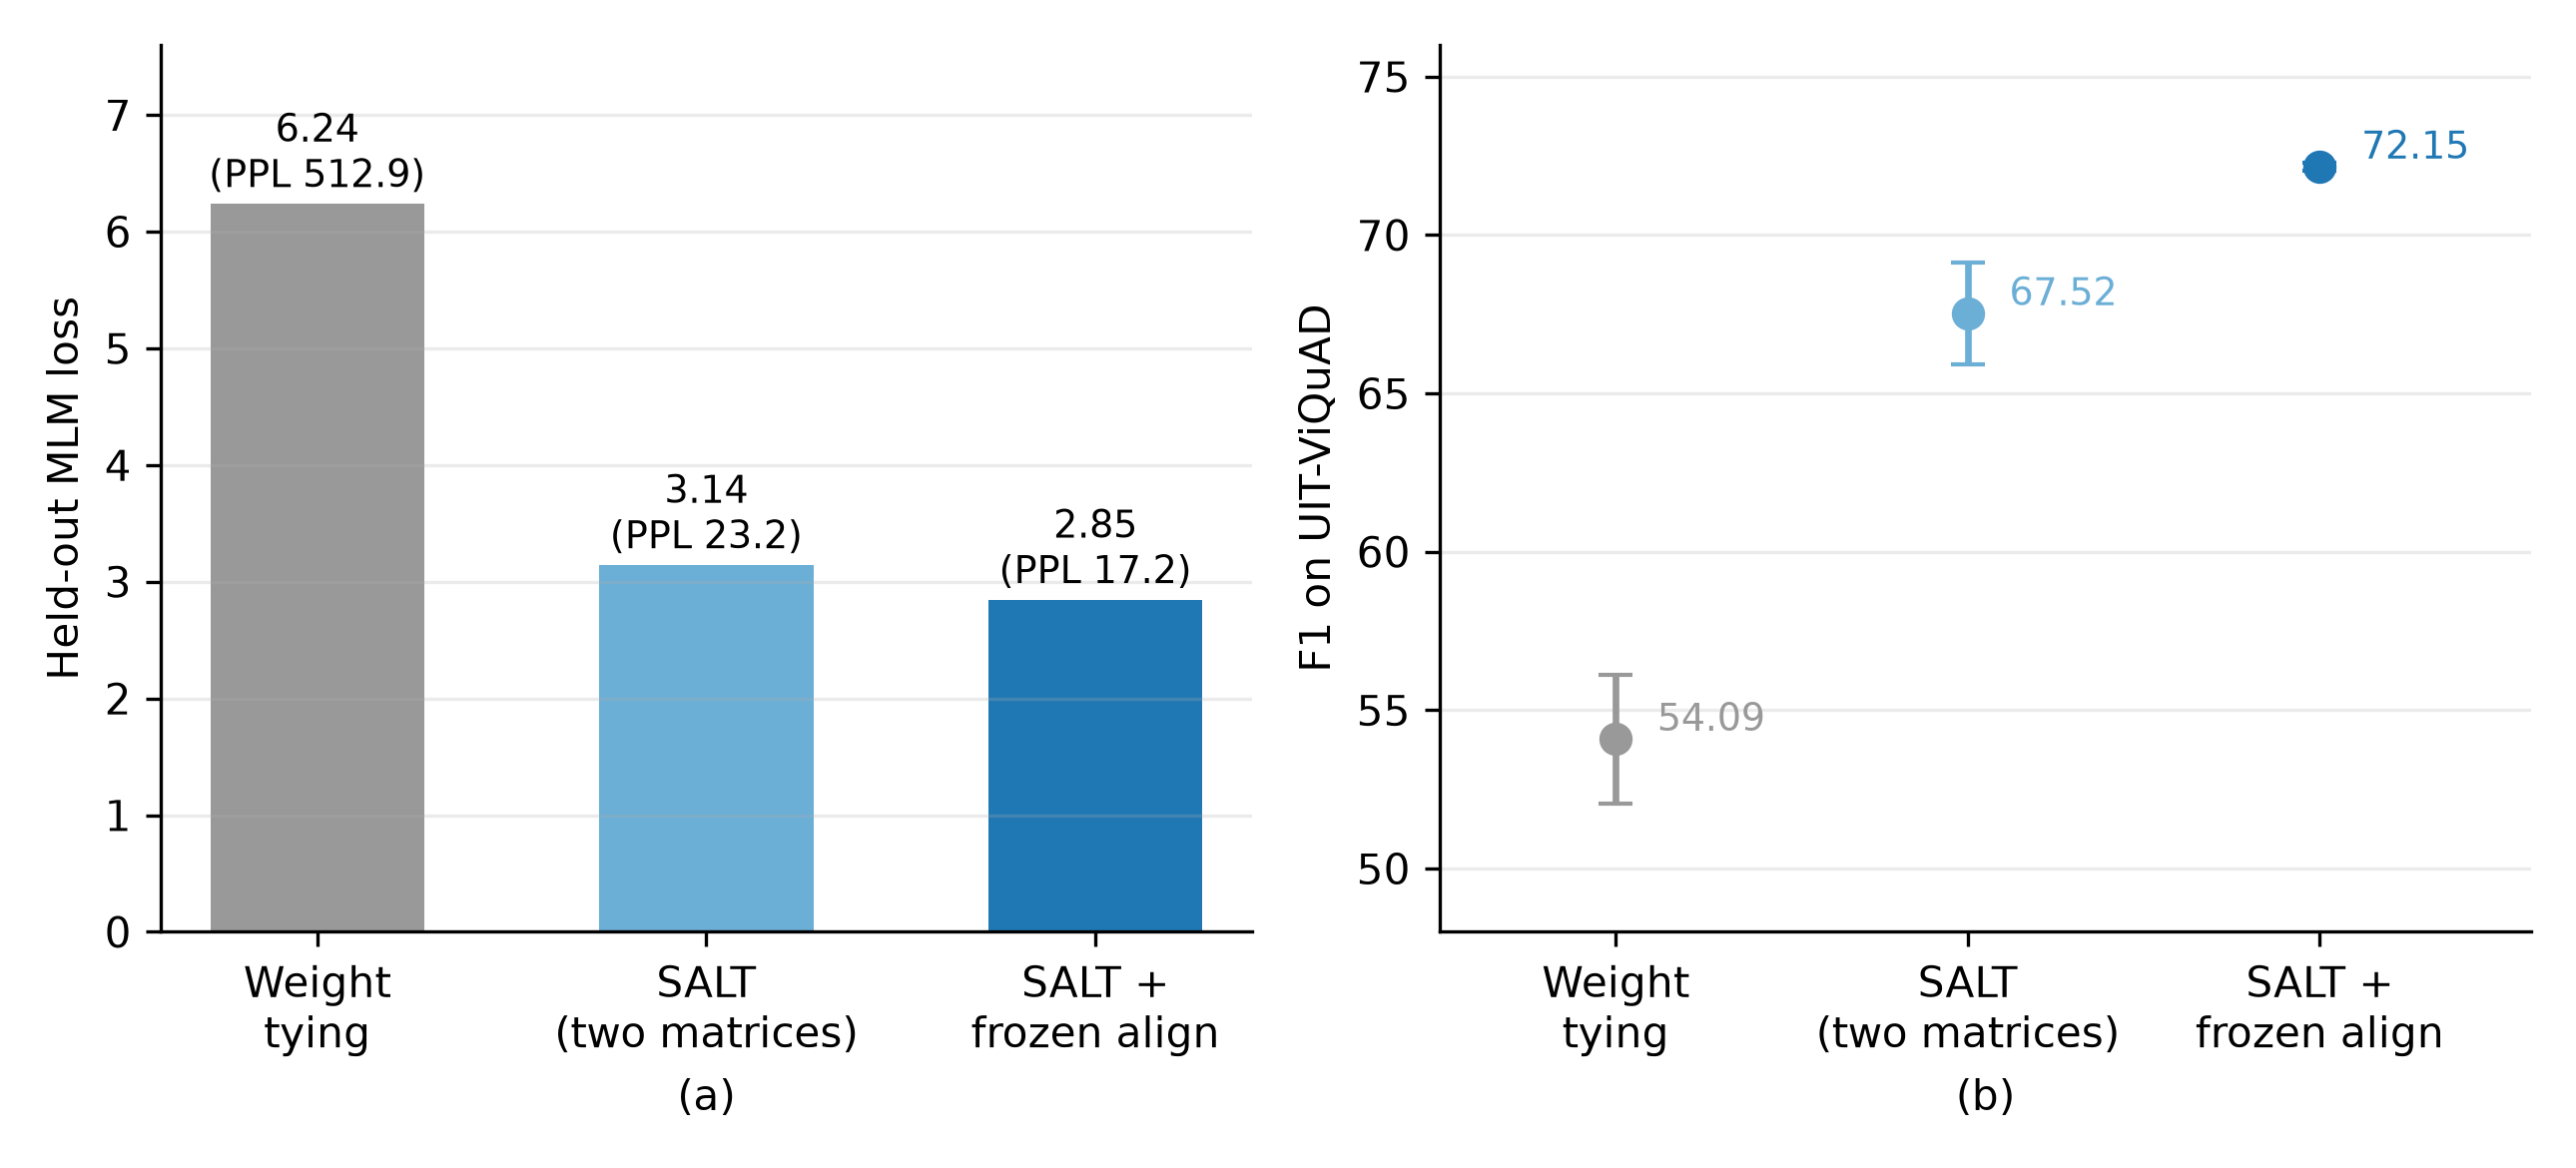
\includegraphics[width=0.95\textwidth]{images/init_strategy_100k.png}
  \caption{So sánh năm phương án khởi tạo theo mất mát MLM/PPL và F1 trên UIT-ViQuAD.}
  \label{fig:init-strategy}
\end{figure}

Biểu đồ bên trái của Hình~\ref{fig:init-strategy} đo khả năng dự đoán token bị che bằng
mất mát MLM và PPL, vì vậy cột càng thấp thì tốt hơn. Biểu đồ bên phải đo khả năng sử
dụng biểu diễn cho bài toán đọc hiểu UIT-ViQuAD bằng điểm F1, vì vậy điểm càng cao thì
tốt hơn. Hai biểu đồ cần được đọc đồng thời để tránh lựa chọn một phương án chỉ có mất
mát MLM thấp nhưng chưa tạo ra biểu diễn ngữ nghĩa hữu ích cho tác vụ thực tế.

Trước hết, so sánh hai phương án ``Naive random'' và ``Norm-matched random'' cho thấy tác
dụng của việc đưa độ lớn véc-tơ về đúng mức. Naive random chỉ đạt
$43{,}51 \pm 3{,}03$ F1 và có mất mát 5,49, tương ứng PPL 242,9; trong khi
Norm-matched random tăng lên $56{,}27 \pm 0{,}79$ F1 và giảm mất mát còn 3,48, tương
ứng PPL 32,4. Nhận xét về lợi ích của khớp mô-men vì vậy được rút ra trực tiếp từ chênh
lệch giữa hai nhãn này trên cả biểu đồ bên trái và biểu đồ bên phải.

Tiếp theo, so sánh ``Norm-matched random'' với ``SALT (both)'' cho phép tách riêng giá
trị của hướng ngữ nghĩa mà SALT chuyển giao. SALT (both) đạt
$67{,}52 \pm 1{,}61$ F1 và mất mát 3,14, tương ứng PPL 23,2, cao hơn
Norm-matched random khoảng 11,2 điểm F1. Do cả hai phương án đều đã xử lý độ lớn, ánh xạ
đầu ra và tần suất token, chênh lệch giữa hai nhãn này chủ yếu phản ánh lợi ích của hướng
véc-tơ ngữ nghĩa được tái sử dụng từ mô hình nguồn.

Đối với phương án ``Weight tying'', kết quả $54{,}09 \pm 2{,}04$ F1 và mất mát 6,24,
tương ứng PPL 512,9, thấp hơn cả ``Norm-matched random'' về F1 và kém rõ rệt so với
``SALT (both)''. Kết luận rằng không nên dùng chung trọng số được rút ra từ chính sự đối
chiếu Weight tying với hai nhãn này. Nguyên nhân là ma trận đầu vào và ma trận đầu ra của
NeoBERT đảm nhiệm hai vai trò hình học khác nhau (Mục~\ref{sec:geometry}), do đó việc
buộc chúng dùng chung một ma trận ngay từ khởi tạo làm giảm chất lượng thay vì tạo ra lợi
ích.

Lợi ích của pha căn chỉnh được xác định bằng cách so sánh trực tiếp ``SALT (both)'' với
``SALT + freeze''. Khi thêm pha căn chỉnh với phần thân đóng băng, mất mát giảm từ 3,14
xuống 2,85, PPL giảm từ 23,2 xuống 17,2, F1 tăng từ 67,52 lên 72,15 và độ lệch chuẩn
giảm từ 1,61 xuống 0,12. Do hai nhãn chỉ khác nhau ở pha căn chỉnh khoảng 20 triệu token,
mức cải thiện này cho thấy đây là một bước bổ sung hiệu quả và giúp kết quả ổn định hơn.

Cuối cùng, việc đối chiếu ``Norm-matched random'' với ``SALT (both)'' giữa hai biểu đồ
cho thấy không thể lựa chọn chiến lược chỉ dựa trên mất mát MLM. Ở biểu đồ bên trái, mất
mát của Norm-matched random là 3,48, khá gần SALT (both) ở mức 3,14; tuy nhiên, ở biểu
đồ bên phải, F1 của Norm-matched random thấp hơn SALT (both) hơn 11 điểm. Nhận xét này
cho thấy mất mát MLM chủ yếu phản ánh khả năng dự đoán token, còn UIT-ViQuAD buộc mô
hình sử dụng quan hệ ngữ nghĩa theo ngữ cảnh và vì vậy là tiêu chí cần thiết để lựa chọn
cấu hình cuối.

Tổng hợp các so sánh trong Hình~\ref{fig:init-strategy} cho thấy phương án tốt nhất là
khởi tạo SALT riêng cho ma trận đầu vào và ma trận đầu ra với $\gamma = 0{,}1$, sau đó
căn chỉnh hai ma trận trên phần thân NeoBERT đóng băng trước khi tiếp tục tiền huấn
luyện. Phương án này tương ứng với nhãn ``SALT + freeze'' trong hình và đồng thời đạt
mất mát MLM/PPL thấp nhất, F1 UIT-ViQuAD cao nhất cùng độ ổn định tốt nhất trong năm
phương án. Do đó, đây là cấu hình khởi tạo được sử dụng cho ViNeoBERT.

% ======================================================================
\section{Kết quả của mô hình cuối}
\label{sec:exp-mrc}

Sau khi lựa chọn được phương án khởi tạo ở Mục~\ref{sec:exp-bakeoff}, mô hình được tiếp
tục tiền huấn luyện trên khoảng 5 tỷ token tiếng Việt từ
CulturaX~\cite{nguyen2023culturax} theo lịch WSD (Mục~\ref{sec:cpt}). Bài toán của mục
này là xác định việc tái sử dụng lớp véc-tơ được khởi tạo bằng SALT và phần thân NeoBERT
đã huấn luyện có tạo ra một mô hình tiếng Việt hiệu quả hay không. Đầu vào của quá trình
đánh giá gồm các điểm kiểm tra được lưu theo lượng token đã huấn luyện và điểm kiểm tra
cuối ở mốc 5 tỷ token; đầu ra gồm đường cong mất mát, kết quả đọc hiểu UIT-ViQuAD và điểm
số trên mười hai tác vụ thuộc nhiều nhóm năng lực. Các kết quả được đối chiếu với
PhoBERT-base-v2, PhoBERT-large~\cite{nguyen2020phobert}, XLM-R-base và
XLM-R-large~\cite{conneau2020xlmr}. Phần đánh giá được trình bày theo ba bước:
Mục~\ref{subsec:exp-curve} xem xét tốc độ hình thành chất lượng theo lượng dữ liệu;
Mục~\ref{subsec:exp-multitask} phân tích mô hình cuối theo từng nhóm năng lực; và
Mục~\ref{subsec:exp-ctx4096} kiểm tra khả năng sử dụng ngữ cảnh dài sau pha mở rộng lên
4.096 token.

\subsection{Chất lượng theo lượng dữ liệu huấn luyện}
\label{subsec:exp-curve}

Trước hết, thí nghiệm cần trả lời hai câu hỏi có liên hệ trực tiếp với nhau: quá trình
tiếp tục tiền huấn luyện có hội tụ ổn định hay không, và chất lượng thu được có chuyển
thành năng lực xử lý tác vụ thực tế hay không. Với câu hỏi thứ nhất, đầu vào là các điểm
kiểm tra của ViNeoBERT từ khoảng 0,1 đến 5 tỷ token; đầu ra là mất mát MLM trên tập huấn
luyện, mất mát trên tập đánh giá và perplexity tương ứng. Mất mát và perplexity càng thấp
thì mô hình càng gán xác suất cao cho token đúng. Hình~\ref{fig:cpt-loss} trình bày đồng
thời diễn biến trên tập huấn luyện và tập đánh giá để có thể phân biệt sự cải thiện thực
sự với hiện tượng chỉ khớp dữ liệu huấn luyện.

\begin{figure}[tbp]
  \centering
  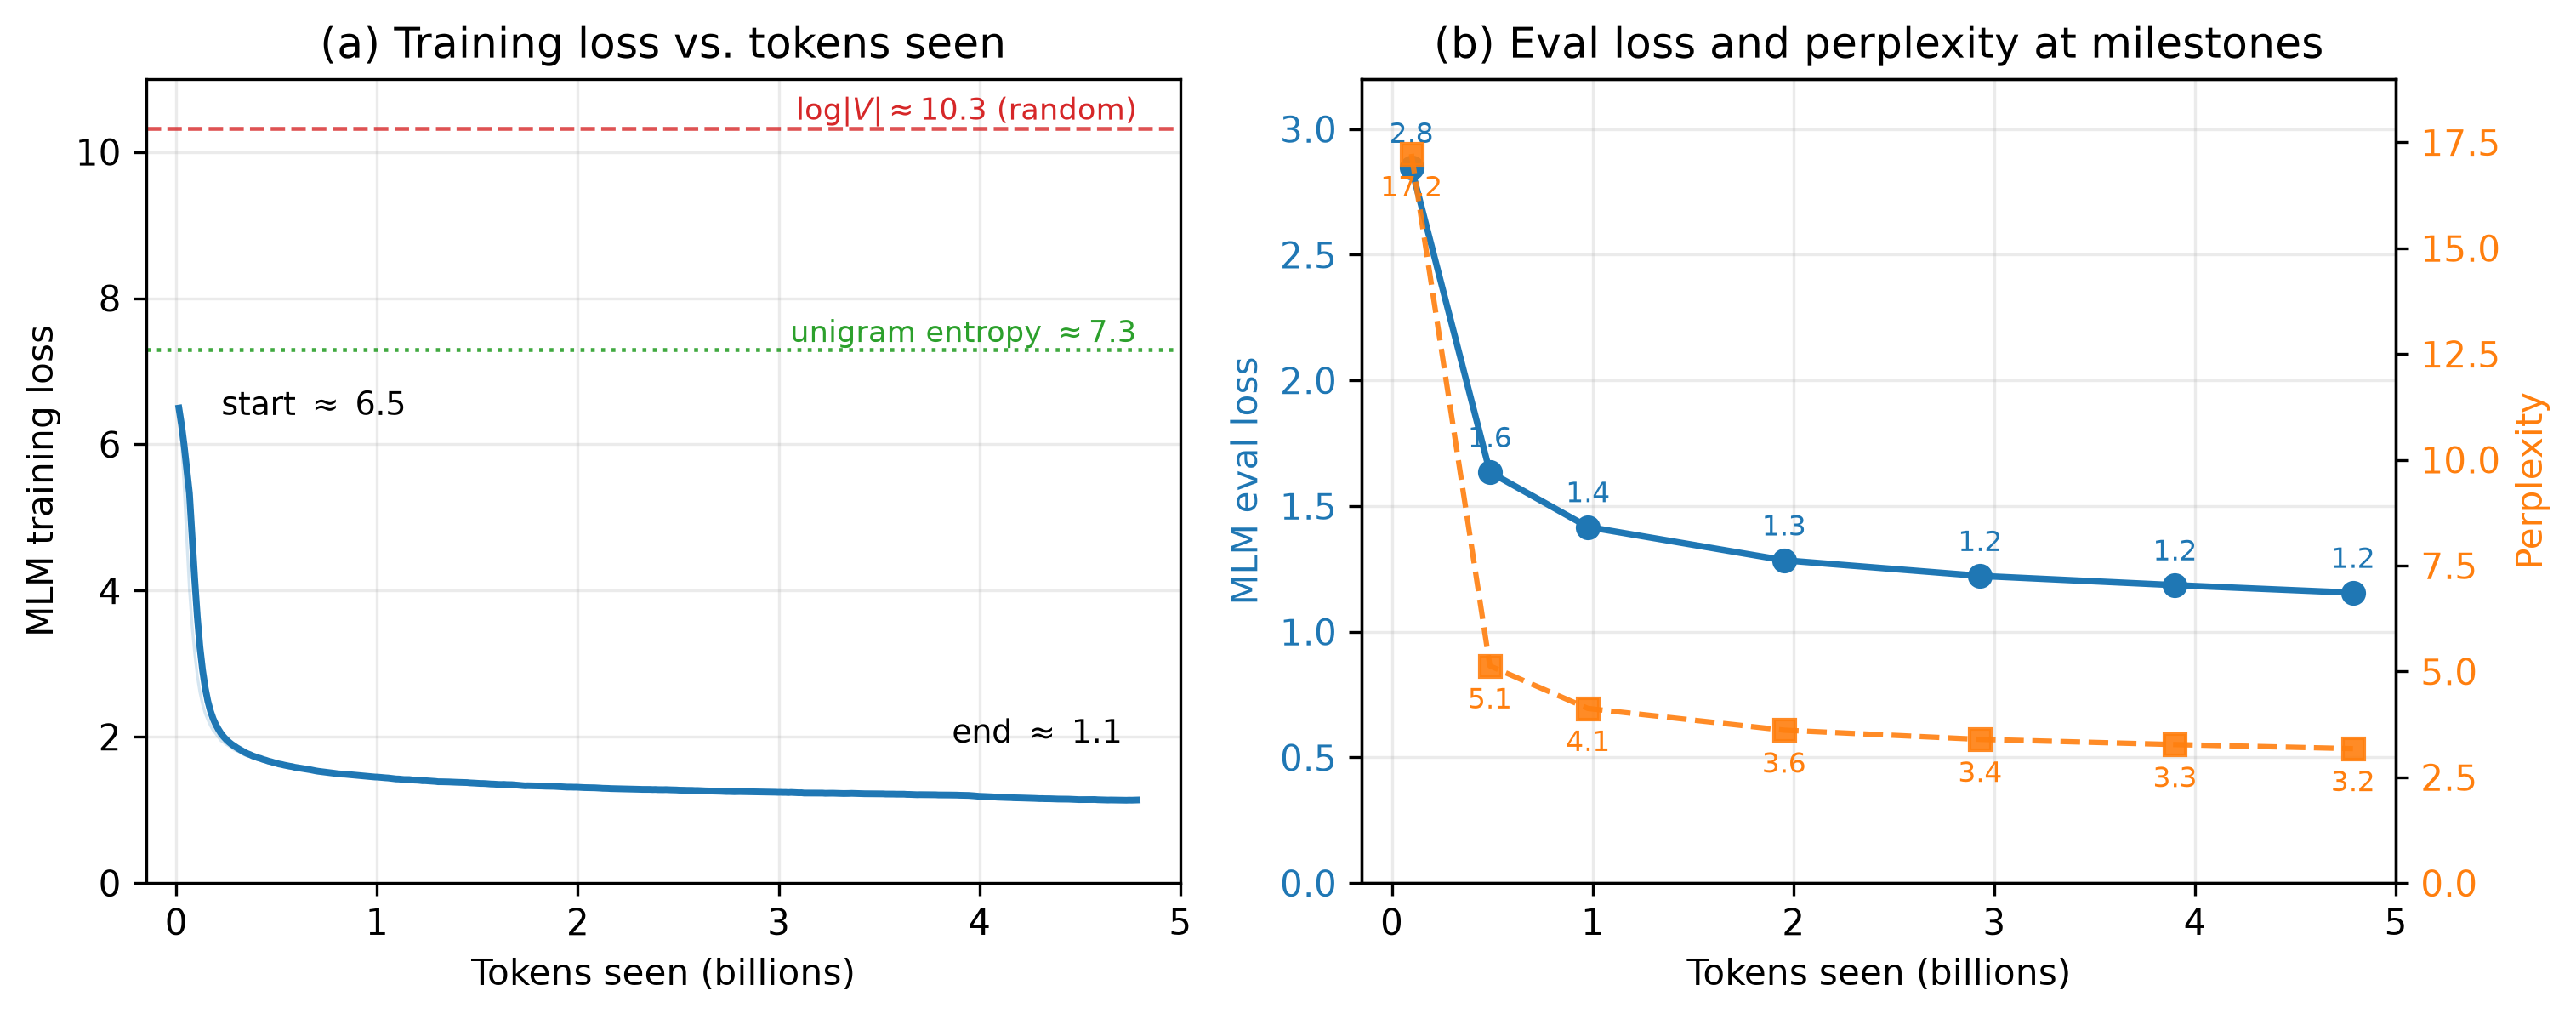
\includegraphics[width=\textwidth]{images/cpt_loss_curve.png}
  \caption{Đường cong mất mát giai đoạn CPT theo lịch WSD.}
  \label{fig:cpt-loss}
\end{figure}

Biểu đồ bên trái của Hình~\ref{fig:cpt-loss} có trục ngang là số token đã thấy và trục
dọc là mất mát MLM. Hai đường tham chiếu giúp xác định chất lượng của điểm xuất phát:
$\log|\mathcal{V}_t| \approx 10{,}3$ là mức của dự đoán gần như ngẫu nhiên, còn entropy
unigram $\approx 7{,}3$ là mức có thể đạt được khi chủ yếu dựa vào tần suất token tiếng
Việt. ViNeoBERT bắt đầu ở khoảng 6,5, thấp hơn cả hai mốc này, sau đó mất mát giảm xuống
dưới 2,0 chỉ trong khoảng 0,2 tỷ token đầu và kết thúc quanh 1,1. Biểu đồ bên phải cho
thấy cùng xu hướng trên dữ liệu không dùng để cập nhật trọng số: mất mát đánh giá giảm
từ 2,8 xuống khoảng 1,2, còn perplexity giảm từ 17,2 ở mốc khoảng 0,1 tỷ token xuống 3,3
ở khoảng 3,9 tỷ token và 3,2 ở điểm kiểm tra cuối. Việc cả hai đường cùng giảm cho thấy
mô hình không chỉ ghi nhớ tập huấn luyện mà đang thích nghi ổn định với phân phối tiếng
Việt.

Tuy nhiên, mất mát MLM thấp chưa đủ để kết luận mô hình xử lý tốt tác vụ ứng dụng. Vì
vậy, tại mỗi mốc ngân sách, một nhánh của mô hình được làm nguội rồi tinh chỉnh trên
UIT-ViQuAD. Trong tác vụ này, đầu vào là một đoạn văn cùng câu hỏi, còn đầu ra là vị trí
bắt đầu và kết thúc của câu trả lời trong đoạn văn. Điểm F1 đo mức độ trùng khớp token
giữa câu trả lời dự đoán và đáp án chuẩn, do đó cho điểm một phần khi mô hình xác định
đúng phần lớn nhưng chưa khớp hoàn toàn (Mục~\ref{sec:exp-metrics}).
Hình~\ref{fig:mrc-curve} biểu diễn điểm F1 theo lượng token tiếp tục tiền huấn luyện;
đường càng cao thì khả năng đọc và định vị câu trả lời càng tốt.

\begin{figure}[tbp]
  \centering
  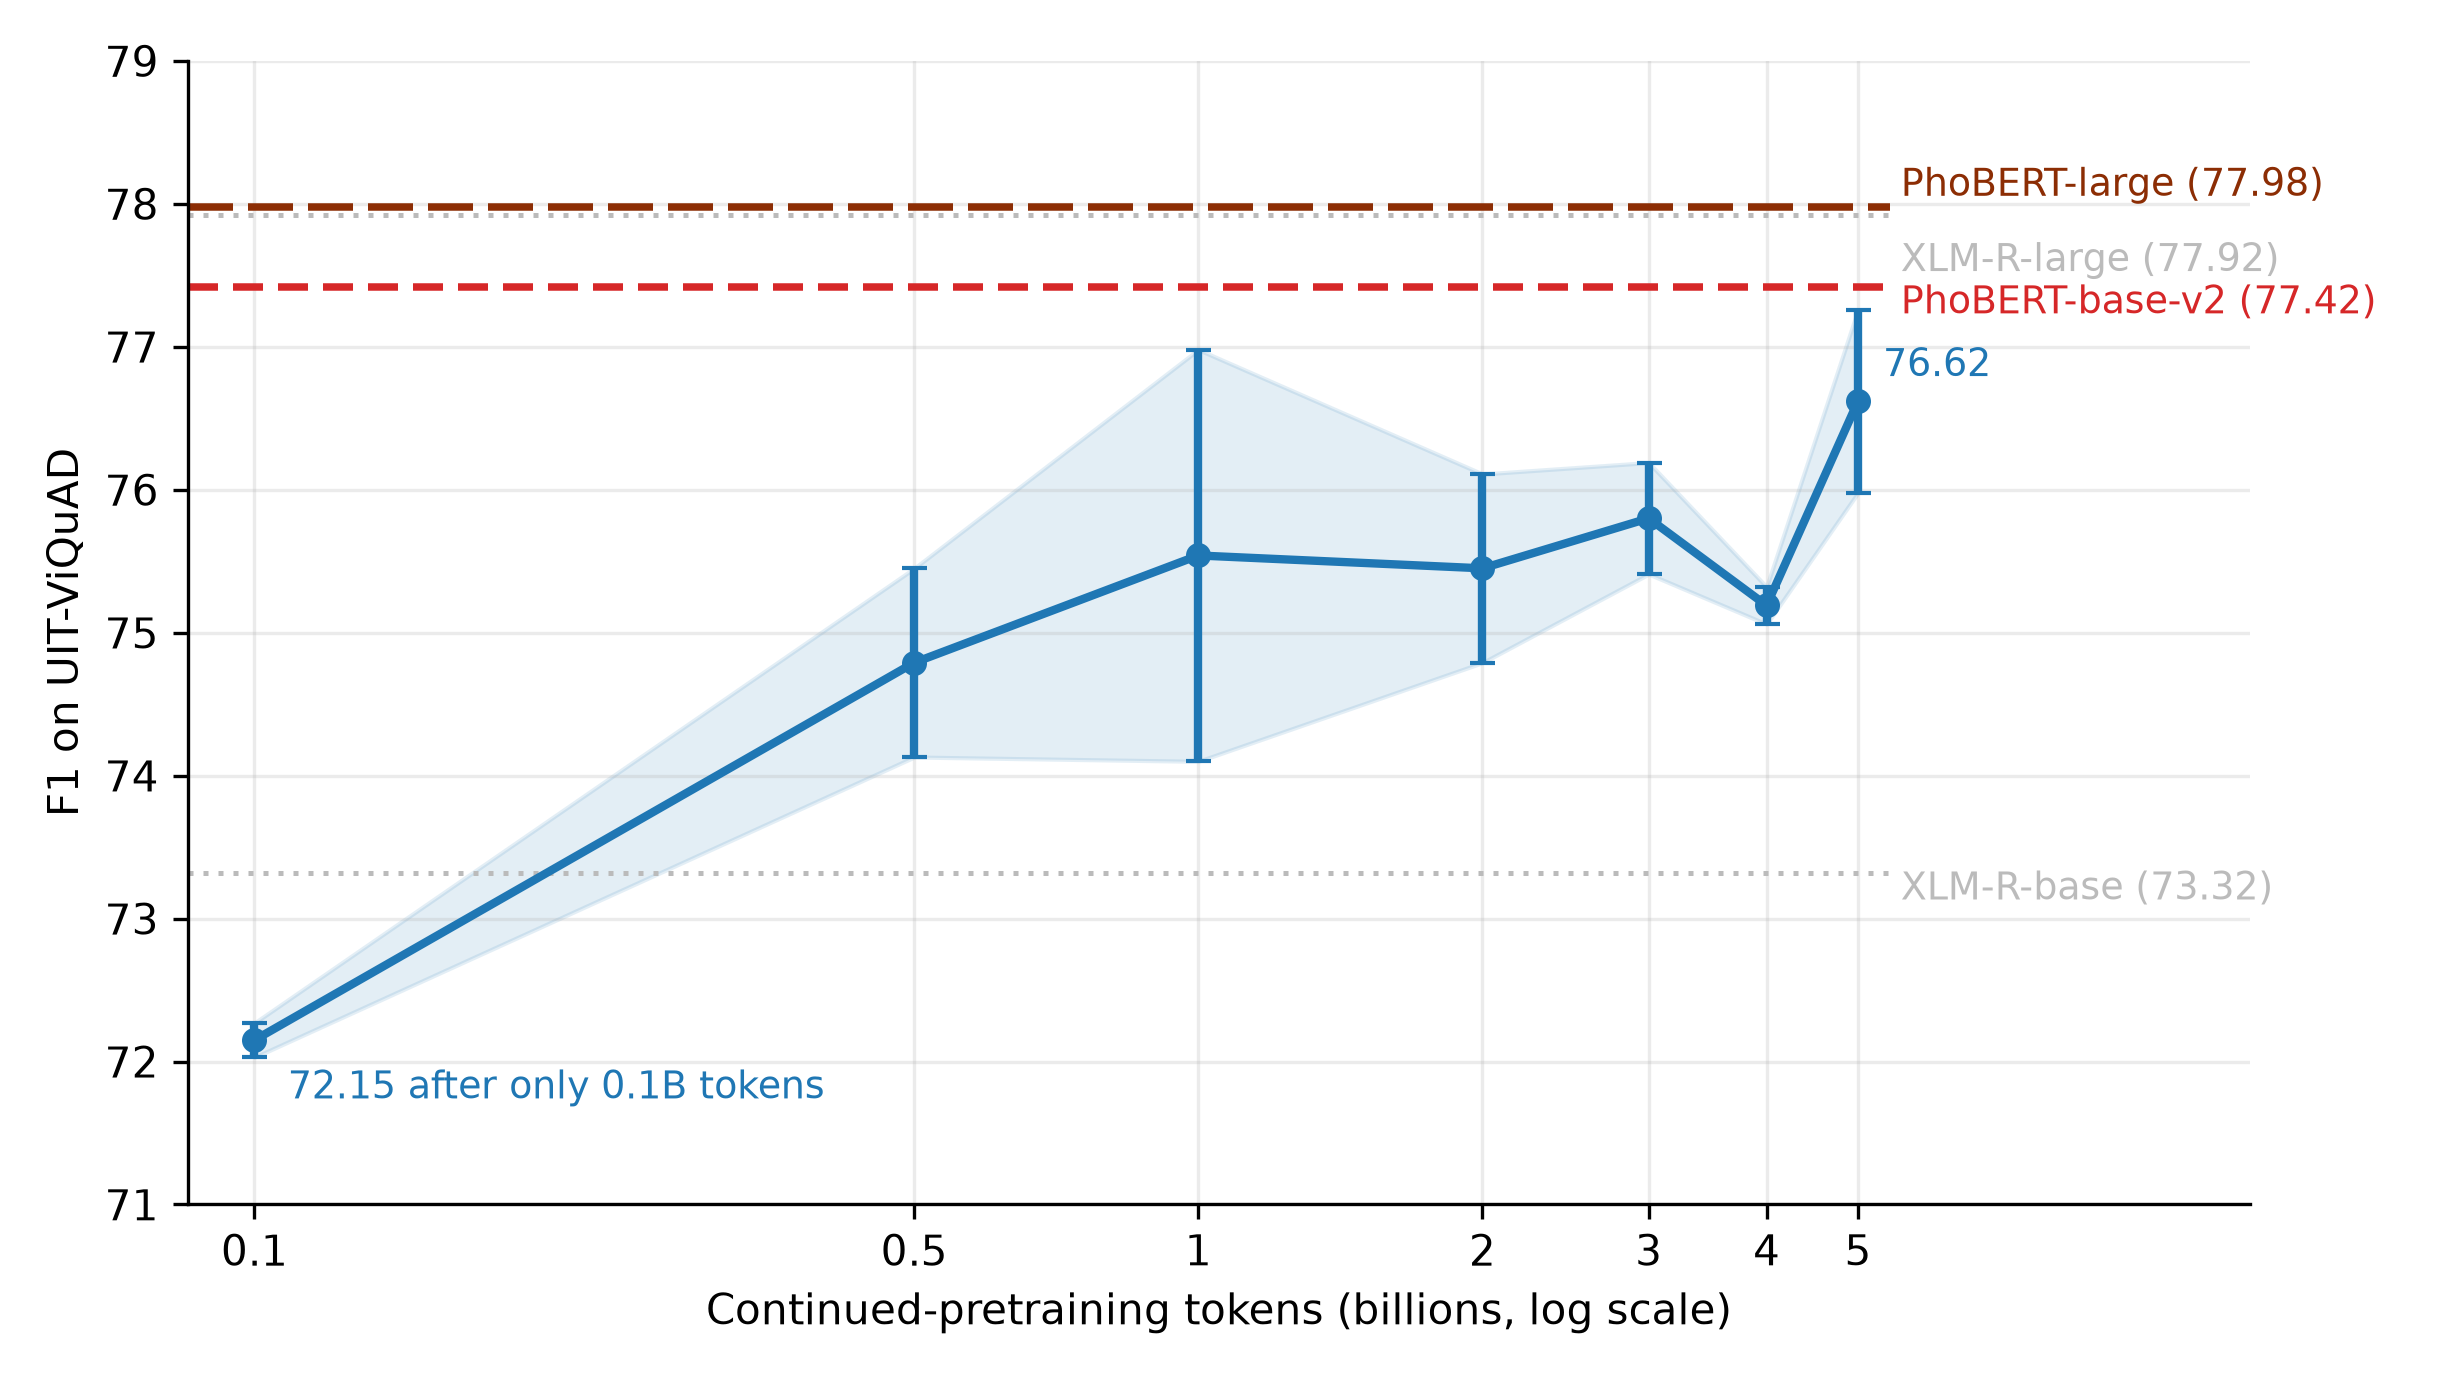
\includegraphics[width=0.92\textwidth]{images/mrc_curve_tokens.png}
  \caption{Điểm F1 trên UIT-ViQuAD theo số token CPT.}
  \label{fig:mrc-curve}
\end{figure}

Hình~\ref{fig:mrc-curve} cho thấy chất lượng ứng dụng xuất hiện khá sớm. Ở mốc 0,1 tỷ
token, tương đương khoảng 2\% ngân sách, ViNeoBERT đã đạt 72,15 F1 và chỉ còn cách kết
quả cuối 4,47 điểm. Đến 0,5 tỷ token, điểm số tăng lên 74,79 và vượt kết quả cuối của
XLM-R-base là 73,32. Từ 1 đến 4 tỷ token, đường cong dao động trong khoảng 75--76 điểm;
sau pha làm nguội ở mốc 5 tỷ token, điểm F1 tăng lên 76,62. Kết quả cuối thấp hơn
PhoBERT-base-v2 0,80 điểm và PhoBERT-large 1,36 điểm, nhưng khoảng cách này nhỏ nếu đặt
cạnh chênh lệch rất lớn về lượng dữ liệu huấn luyện.

Bảng~\ref{tab:tokens-seen} đặt các kết quả trên trong cùng bối cảnh ngân sách dữ liệu.
Giá trị ở cột cuối là tổng lượng token mô hình đã thấy trong quá trình tiền huấn luyện,
không chỉ là kích thước kho ngữ liệu ban đầu. Cách phân biệt này đặc biệt quan trọng vì
PhoBERT đi qua cùng kho dữ liệu nhiều epoch~\cite{nguyen2020phobert}, trong khi
ViNeoBERT chỉ đi qua khoảng 5 tỷ token tiếng Việt một lượt; số liệu XLM-R được tổng hợp
từ giao thức huấn luyện và kho CC-100~\cite{conneau2020xlmr}.

\begin{table}[ht]
  \caption{Lượng dữ liệu tiếng Việt đã xử lý.}
  \label{tab:tokens-seen}
  \centering
  \small
  \resizebox{\textwidth}{!}{%
  \begin{tabular}{lll}
    \hline
    \textbf{Mô hình} & \textbf{Kho ngữ liệu} & \textbf{Token đã thấy} \\
    \hline
    PhoBERT (base/large) & 20GB ($\sim$3,5 tỷ token) & $\sim$140 tỷ (40 epoch) \\
    PhoBERT-base-v2      & 140GB ($\sim$25 tỷ token) & không công bố ($\geq$ bản gốc) \\
    XLM-R (base/large)   & CC-100 2,5TB; phần vi 24,76 tỷ token & $\sim$6.300 tỷ (đa ngôn ngữ); vi ước hàng trăm tỷ \\
    ViNeoBERT            & 20GB ($\sim$5 tỷ token)   & 5 tỷ (một lượt) \\
    \hline
  \end{tabular}%
  }
\end{table}

ViNeoBERT chỉ đi qua 5 tỷ token trong một lượt, xấp xỉ 3,5\% lượng token mà
PhoBERT-large đã thấy, nhưng
đạt 99,0\% điểm F1 của PhoBERT-base-v2 và 98,3\% của PhoBERT-large trên UIT-ViQuAD. Từ
đó có thể kết luận rằng đọc hiểu là một năng lực tốt của ViNeoBERT xét theo hiệu quả dữ
liệu: mô hình chưa đứng đầu về điểm tuyệt đối, nhưng đã tiến sát các mô hình đơn ngữ
được huấn luyện với ngân sách lớn hơn nhiều. Đường cong tăng nhanh ngay từ giai đoạn đầu
cũng phù hợp với vai trò của SALT: lớp véc-tơ tiếng Việt được đưa vào vùng biểu diễn mà
NeoBERT đã quen xử lý, nhờ đó mô hình có thể tái sử dụng tri thức của phần thân thay vì
phải hình thành lại toàn bộ năng lực đọc hiểu từ đầu.

\subsection{Đánh giá đa tác vụ}
\label{subsec:exp-multitask}

Kết quả trên một tác vụ đọc hiểu chưa đủ để mô tả đầy đủ mô hình. Vì vậy, bài toán ở
Mục~\ref{subsec:exp-multitask} là xác định ViNeoBERT mạnh và yếu ở những năng lực nào khi
cùng một điểm kiểm tra 5 tỷ token được đưa sang nhiều loại dữ liệu khác nhau. Đầu vào
của thí nghiệm gồm điểm kiểm tra cuối và tập dữ liệu của mười hai tác vụ
(Mục~\ref{subsec:exp-eval-data}); đầu ra có thể là nhãn của cả câu, nhãn của từng token,
mức tương đồng giữa hai câu hoặc danh sách tài liệu được xếp hạng. Các đầu ra này được
quy đổi thành độ đo phù hợp với từng tác vụ như Accuracy, F1, MCC, Spearman, nDCG@10 và
MRR. Dấu mũi tên hướng lên trong Bảng~\ref{tab:multitask} cho biết mọi độ đo đều được
đọc theo cùng một hướng: giá trị càng cao càng tốt. Các tác vụ có bước tinh chỉnh được
báo cáo bằng giá trị trung bình của năm seed. Riêng Retrieval và Reranking chỉ dùng để
đánh giá, không có quá trình tinh chỉnh theo seed, nên mỗi mô hình được đánh giá một lần
theo cùng một giao thức cố định (Mục~\ref{sec:exp-metrics}).

\begin{table}[ht]
  \caption{Kết quả đánh giá đa tác vụ tại điểm kiểm tra 5 tỷ token (giá trị tốt nhất in đậm).}
  \label{tab:multitask}
  \centering
  \small
  \resizebox{\textwidth}{!}{%
  \begin{tabular}{llcccc>{\columncolor{ourcol}}c}
    \hline
    \textbf{Tác vụ} & \textbf{Độ đo} & \textbf{PhoBERT-base-v2} & \textbf{PhoBERT-large} & \textbf{XLM-R-base} & \textbf{XLM-R-large} & \textbf{ViNeoBERT} \\
    \hline
    UIT-VSFC         & F1-weighted ($\uparrow$) & 0,9345 & \textbf{0,9356} & 0,9281 & 0,9312 & 0,9284 \\
    UIT-VSMEC        & F1-macro ($\uparrow$)    & \textbf{0,6415} & 0,6132 & 0,6145 & 0,3125 & 0,6163 \\
    UIT-ViCTSD       & F1-macro ($\uparrow$)    & 0,7455 & \textbf{0,7526} & 0,7110 & 0,5759 & 0,7315 \\
    ViCoLA-syn       & MCC ($\uparrow$)         & \textbf{0,8103} & 0,7915 & 0,7827 & 0,4845 & 0,7789 \\
    XNLI (vi)        & Accuracy ($\uparrow$)    & 0,7720 & 0,7769 & 0,7541 & \textbf{0,8000} & 0,7714 \\
    ViANLI           & F1-macro ($\uparrow$)    & \textbf{0,4529} & 0,3882 & 0,3625 & 0,1666 & 0,4273 \\
    QNLI (vi)        & Accuracy ($\uparrow$)    & 0,8872 & 0,8861 & 0,8592 & \textbf{0,8940} & 0,8791 \\
    UD-VTB (POS)     & F1-macro ($\uparrow$)    & 0,7799 & 0,7879 & 0,7827 & 0,8062 & \textbf{0,8089} \\
    STS (vi)         & Spearman ($\uparrow$)    & 0,8557 & 0,8509 & 0,8226 & \textbf{0,8644} & 0,8392 \\
    Paraphrase (STS) & F1-macro ($\uparrow$)    & 0,9351 & 0,9400 & 0,9016 & \textbf{0,9437} & 0,9276 \\
    Retrieval (ViQuAD)  & nDCG@10 ($\uparrow$) & \textbf{0,4719} & 0,4659 & 0,1386 & 0,2565 & 0,4061 \\
    Reranking (ViQuAD)  & MRR ($\uparrow$)     & \textbf{0,8922} & 0,8794 & 0,5282 & 0,6741 & 0,8448 \\
    \hline
  \end{tabular}%
  }
\end{table}

Trước khi phân tích theo từng nhóm năng lực, cần xác định mốc so sánh phù hợp.
PhoBERT-base-v2 và XLM-R-base gần ViNeoBERT hơn về quy mô tham số, còn hai mô hình
\texttt{large} chủ yếu cho biết mức điểm có thể đạt được khi tăng đáng kể kích thước mô
hình. Vì vậy, phần giải thích dưới đây ưu tiên khoảng cách với PhoBERT-base-v2 và vị trí
của ViNeoBERT trong cả năm mô hình. Theo Bảng~\ref{tab:multitask}, ViNeoBERT cao hơn
XLM-R-base ở 11 trong 12 tác vụ; ngoại lệ duy nhất là ViCoLA-syn, nơi hai mô hình chỉ
chênh 0,0038 điểm.

Ở nhóm phân loại một câu, gồm UIT-VSFC, UIT-VSMEC và UIT-ViCTSD, kết quả nhìn chung ở
mức cạnh tranh nhưng chưa dẫn đầu. ViNeoBERT đạt lần lượt 0,9284, 0,6163 và 0,7315,
tương ứng đứng hạng 4, hạng 2 và hạng 3 trong năm mô hình. Khoảng cách tương đối so với
mô hình tốt nhất ở từng tác vụ lần lượt chỉ khoảng 0,77\%, 3,93\% và 2,80\%. Điều này
cho thấy các biểu diễn được chuyển giao đã hỗ trợ tốt việc nhận biết chủ đề, cảm xúc và
nội dung độc hại ở mức tổng quát. Tuy nhiên, việc mô hình chưa đứng đầu cũng cho thấy
những tín hiệu rất đặc thù của tiếng Việt như từ lóng, mỉa mai, cách biểu đạt cảm xúc
hiếm hoặc ngữ cảnh văn hóa chưa được kế thừa đầy đủ từ tri thức tiếng Anh.

Hai tác vụ liên quan đến cấu trúc ngôn ngữ cho kết quả trái chiều và cần được tách thành
hai năng lực khác nhau. Trên UD-VTB POS, mô hình phải gán nhãn từ loại cho từng token;
ViNeoBERT đạt 0,8089 và đứng đầu cả năm mô hình, cao hơn XLM-R-large 0,0027 điểm. Đây là
điểm mạnh rõ nhất trong Bảng~\ref{tab:multitask} và phù hợp với cách SALT chuyển lớp
véc-tơ theo token để phần thân NeoBERT tiếp tục khai thác biểu diễn ngữ cảnh đã học.
Ngược lại, ViCoLA-syn yêu cầu nhận biết một câu có bị làm sai về mặt cú pháp hay không;
ViNeoBERT đạt 0,7789, đứng hạng 4/5 và thấp hơn PhoBERT-base-v2 0,0314 điểm, tương
đương 3,88\%. Kết quả này cho thấy mô hình nhận biết vai trò của từng từ rất tốt nhưng
còn yếu hơn khi phải phát hiện các biến đổi cấp câu như đảo, bỏ hoặc lặp cụm từ. Vì vậy,
không thể từ kết quả POS suy rộng rằng mô hình đã mạnh ở toàn bộ năng lực ngữ pháp.

Ở nhóm đọc hiểu và suy luận, các kết quả cho thấy một xu hướng tích cực. Đọc hiểu
UIT-ViQuAD đã đạt 76,62 F1 ở Mục~\ref{subsec:exp-curve}. Trên XNLI, ViNeoBERT đạt
0,7714, gần như ngang PhoBERT-base-v2 0,7720 với chênh lệch chỉ 0,0006. XNLI tiếng Việt
được dịch từ dữ liệu tiếng Anh~\cite{conneau2018xnli}, do đó cấu trúc lập luận của bài
toán gần với tri thức mà NeoBERT đã học; kết quả này phù hợp với giả thuyết rằng SALT
giúp tái sử dụng tri thức tiếng Anh sau khi chuyển lớp véc-tơ sang tiếng Việt. Trên
ViANLI, một bộ dữ liệu tiếng Việt bản địa và có tính đối kháng cao
hơn~\cite{huynh2024vianli}, ViNeoBERT đạt 0,4273 và đứng hạng 2/5, chỉ sau
PhoBERT-base-v2 0,4529 nhưng cao hơn PhoBERT-large cùng cả hai mô hình XLM-R. Do đó,
ViANLI là điểm tốt về thứ hạng chứ không phải điểm yếu; khoảng cách 0,0256 với vị trí đầu
chỉ cho thấy các mẫu suy luận đối kháng và sắc thái bản địa vẫn còn dư địa cải thiện.
QNLI đạt 0,8791, thấp hơn PhoBERT-base-v2 0,0081, tiếp tục cho thấy năng lực xác định
quan hệ giữa câu hỏi và câu trả lời ở mức ổn định.

Ở nhóm so khớp ngữ nghĩa, ViNeoBERT đạt 0,8392 Spearman trên STS và 0,9276 F1 trên
Paraphrase-STS. So với PhoBERT-base-v2, mức chênh lần lượt là 0,0165 và 0,0075, đều
dưới 2\% theo tỷ lệ tương đối. Mô hình vì vậy chưa phải lựa chọn tốt nhất về điểm tuyệt
đối, nhưng đã tái sử dụng khá hiệu quả quan hệ ngữ nghĩa giữa hai câu. Kết quả này, kết
hợp với QNLI, cho thấy biểu diễn của ViNeoBERT đủ tốt cho các bài toán so sánh cặp câu,
dù vẫn còn khoảng cách với các mô hình được tiền huấn luyện lâu hơn hoặc có kích thước
lớn hơn.

Điểm yếu rõ nhất xuất hiện ở nhóm tìm kiếm bằng véc-tơ. ViNeoBERT đạt 0,4061 nDCG@10
trên Retrieval và 0,8448 MRR trên Reranking, đều đứng hạng 3/5. So với
PhoBERT-base-v2, Retrieval thấp hơn 0,0658, tương đương 13,94\%, còn Reranking thấp hơn
0,0474, tương đương 5,31\%. Các điểm số này vẫn cao hơn đáng kể hai mô hình XLM-R nhưng
không hỗ trợ kết luận rằng ViNeoBERT mạnh ở truy hồi. Một cách giải thích phù hợp là
SALT chuyển giao trực tiếp lớp véc-tơ ở cấp token, trong khi tìm kiếm đòi hỏi toàn bộ câu
hoặc đoạn văn phải được nén thành các véc-tơ có khoảng cách toàn cục phù hợp với mức
liên quan. Năng lực thứ hai không tự động được bảo đảm chỉ nhờ các token đã được đặt đúng
vùng biểu diễn, đặc biệt khi dữ liệu tiếng Việt dùng để tiếp tục tiền huấn luyện mới dừng
ở 5 tỷ token.

Tổng hợp các kết quả, ViNeoBERT có điểm mạnh rõ nhất ở gán nhãn từ loại và thể hiện tốt
ở đọc hiểu, suy luận. Phân loại một câu và so khớp cặp câu đạt mức cạnh tranh, với khoảng
cách nhỏ so với PhoBERT-base-v2, nhưng chưa phải nhóm dẫn đầu ổn định. Hai điểm yếu cần
ưu tiên cải thiện là ngữ pháp cấp câu trên ViCoLA-syn và tìm kiếm trực tiếp bằng
véc-tơ trên Retrieval/Reranking. Hồ sơ năng lực này phù hợp với cơ chế chuyển giao
của SALT: tri thức tiếng Anh và biểu diễn theo ngữ cảnh ở cấp token được tái sử dụng
hiệu quả, trong khi các hiện tượng cú pháp bản địa và hình học véc-tơ toàn câu cần
thêm tín hiệu tiếng Việt chuyên biệt.

\subsection{Mở rộng ngữ cảnh lên 4.096 token}
\label{subsec:exp-ctx4096}

Bên cạnh chất lượng trên các tác vụ ngữ cảnh ngắn, thí nghiệm cuối kiểm tra liệu giới
hạn 4.096 token mà ViNeoBERT kế thừa từ kiến trúc
NeoBERT~\cite{lebreton2025neobert} có thực sự sử dụng được hay chỉ tồn tại về mặt cấu
hình. Trong giai đoạn CPT chính, mô hình chỉ được huấn luyện với chuỗi dài 1.024 token;
vì vậy điểm kiểm tra 5 tỷ token được huấn luyện bổ sung khoảng 200 triệu token trên các
chuỗi 4.096 token lấy từ phần dữ liệu CulturaX chưa từng thấy, với tốc độ học cố định
$10^{-5}$ (Bảng~\ref{tab:hyperparams}). Đầu vào của phép đánh giá là các văn bản
Wikipedia tiếng Việt dài từ 1.000 đến 4.096 token. Đầu ra là
\textit{pseudo-perplexity} (PPPL) của cùng tập văn bản trước và sau pha mở rộng, qua đó
xác định chất lượng có suy giảm khi độ dài chuỗi tăng hay không.

PPPL là biến thể của perplexity dành cho mô hình ngôn ngữ có mặt
nạ~\cite{salazar2020mlmscoring}. Thay vì dự đoán token tiếp theo, một vị trí trong chuỗi
được che đi và mô hình phải khôi phục token tại vị trí đó từ phần ngữ cảnh còn lại; xác
suất của các lần khôi phục được tổng hợp thành PPPL. Trong thí nghiệm này, mỗi văn bản
được xấp xỉ bằng 32 vị trí che để giảm chi phí tính toán, và cùng cặp văn bản--độ dài
được dùng cho cả hai điểm kiểm tra. PPPL càng thấp và càng ít tăng theo độ dài thì mô
hình càng duy trì ổn định khả năng sử dụng ngữ cảnh xa.

\begin{figure}[ht]
  \centering
  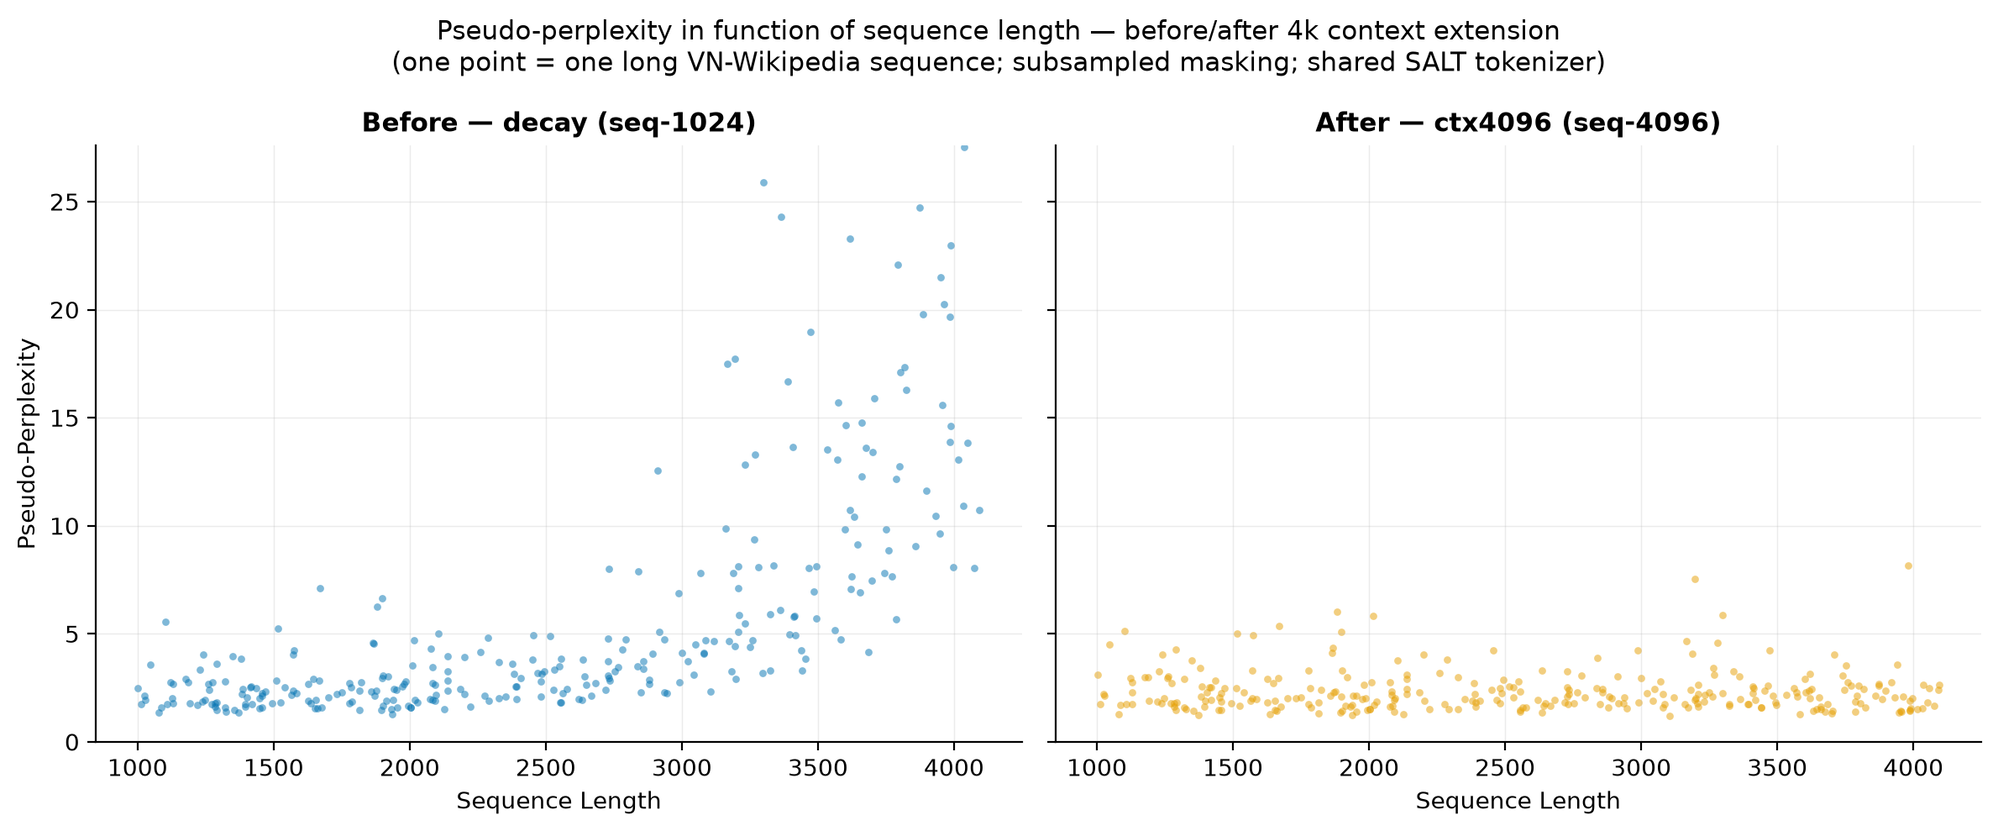
\includegraphics[width=\textwidth]{images/ctx4096_pppl.png}
  \caption{Pseudo-perplexity theo độ dài chuỗi, trước và sau pha mở rộng 4.096 token.}
  \label{fig:ctx4096}
\end{figure}

Hình~\ref{fig:ctx4096} sử dụng trục ngang để biểu diễn độ dài chuỗi và trục dọc để biểu
diễn PPPL, vì vậy các điểm càng thấp và đám mây điểm càng phẳng thì kết quả càng tốt. Ở
biểu đồ bên trái, trước pha mở rộng, PPPL duy trì chủ yếu quanh 2--3 khi độ dài nằm dưới
khoảng 2.500--3.000 token. Sau ngưỡng này, độ phân tán tăng nhanh, nhiều văn bản có PPPL
vượt 10 và một số điểm vượt 25. Điều đó cho thấy RoPE (Mục~\ref{subsec:rope}) giúp mô
hình ngoại suy một phần ra ngoài độ dài 1.024 token đã huấn luyện, nhưng ngữ cảnh quá dài
bắt đầu gây nhiễu thay vì hỗ trợ dự đoán.

Ở biểu đồ bên phải, sau pha mở rộng, phần lớn điểm PPPL nằm quanh 2--3 trên toàn dải tới
4.096 token và không còn xu hướng tăng theo độ dài; chỉ còn một số ít điểm ngoại lệ nhưng
mức tăng nhỏ hơn nhiều so với trước. Từ đó có thể kết luận rằng khoảng 200 triệu token
huấn luyện bổ sung, tương đương gần 4\% ngân sách CPT chính, đã biến giới hạn 4.096 token
kế thừa từ kiến trúc thành khả năng sử dụng ổn định theo độ đo nội tại. Kết luận này chỉ
áp dụng trực tiếp cho PPPL; để khẳng định hiệu quả trên các ứng dụng ngữ cảnh dài như hỏi
đáp đa đoạn hoặc truy xuất tài liệu dài, mô hình vẫn cần được đánh giá bằng các tác vụ
ứng dụng tương ứng.

% ======================================================================
\section{Thảo luận}
\label{sec:exp-discussion}

Các kết quả thực nghiệm nhìn chung phù hợp với mục tiêu đặt ra cho phương pháp. Thí
nghiệm ở Mục~\ref{sec:exp-bakeoff} cho thấy từng lựa chọn trong quá trình khởi tạo đều
tạo ra cải thiện đo được: SALT đưa lớp véc-tơ tiếng Việt về gần vùng không gian mà
NeoBERT quen xử lý khi khoảng cách tâm giảm từ 0,8 xuống 0,3; hệ số
$\gamma = 0{,}1$ giữ ảnh hưởng ban đầu của ma trận đầu ra ở mức phù hợp; khởi tạo SALT
riêng cho hai ma trận đạt 67,52 F1, cao hơn rõ rệt phương án dùng chung trọng số 54,09;
và giai đoạn căn chỉnh với phần thân đóng băng giảm khoảng 26\% perplexity, đồng thời
nâng F1 lên 72,15. Mục~\ref{sec:exp-mrc} tiếp tục cho thấy hiệu quả dữ liệu của cấu hình
này: chỉ với 0,5 tỷ token, ViNeoBERT đã vượt XLM-R-base trên UIT-ViQuAD; đến 5 tỷ token,
mô hình cao hơn XLM-R-base ở 11/12 tác vụ, đạt điểm cao nhất ở UD-VTB POS, đứng hạng 2
trên ViANLI và gần ngang PhoBERT-base-v2 trên XNLI. Kết hợp với 76,62 F1 trên đọc hiểu,
các kết quả cho thấy phần tri thức được kế thừa qua SALT phát huy rõ nhất ở biểu diễn
theo ngữ cảnh cấp token, đọc hiểu và suy luận. Ngoài ra, pha huấn luyện bổ sung khoảng
200 triệu token đã giữ PPPL ổn định tới độ dài 4.096 token, cho thấy trần ngữ cảnh của
kiến trúc có thể được kích hoạt với chi phí tương đối nhỏ.

Dù vậy, kết quả không đồng đều trên mọi năng lực. Nhóm phân loại một câu và so khớp cặp
câu đã cạnh tranh nhưng chưa dẫn đầu ổn định; ViCoLA-syn cho thấy mô hình còn hạn chế ở
ngữ pháp cấp câu; còn Retrieval và Reranking thấp hơn PhoBERT-base-v2 lần lượt khoảng
13,94\% và 5,31\%, nên tìm kiếm bằng véc-tơ vẫn là điểm yếu cần được cải thiện. Những
giới hạn này cần được đặt trong bối cảnh ngân sách tiếp tục tiền huấn luyện mới chỉ là
5 tỷ token, nhỏ hơn đáng kể so với các mô hình so sánh. Vì vậy, kết luận phù hợp nhất
không phải ViNeoBERT mạnh đồng đều trên mọi tác vụ, mà là phương pháp đã chuyển giao hiệu
quả một nhóm năng lực cốt lõi với ngân sách nhỏ, đồng thời chỉ ra rõ hai hướng cần bổ
sung là dữ liệu cú pháp tiếng Việt và tín hiệu huấn luyện cho véc-tơ toàn câu. Các
hạn chế và hướng khắc phục tương ứng được tiếp tục trình bày ở
Mục~\ref{sec:limitations} và Mục~\ref{sec:future-work}.
